\pdfoutput=1
\pdfcompresslevel=9
\pdfinfo
{
    /Author (Autor)
    /Title (Tytul)
    /Subject (Tematyka)
    /Keywords (Slowa kluczowe)
}
%\documentclass[a4paper,polish,onecolumn,oneside,floatssmall,11pt,titleauthor,wide,openright]{mwrep}
%\usepackage[scale={0.7,0.8},paper=a4paper,twoside]{geometry}
\documentclass[a4paper,onecolumn,oneside,12pt,wide,floatssmall]{mwrep}
% \usepackage{polish}
\usepackage{amsmath}
\usepackage{amsfonts}
\usepackage{amssymb}
\usepackage{amsthm}
\usepackage{bookman}
\usepackage{geometry}
\usepackage[utf8x]{inputenc}
\usepackage[T1]{fontenc}
% \usepackage{t1enc}
% \usepackage[pdftex, bookmarks]{hyperref}
\usepackage[pdftex, bookmarks=false]{hyperref}
\def\url#1{{ \tt #1}}

\usepackage{listings}

% marginesy
\textwidth\paperwidth
\advance\textwidth -55mm
\oddsidemargin-0.9in
\advance\oddsidemargin 30mm
\evensidemargin-0.9in
\advance\evensidemargin 30mm
\topmargin -1in
\advance\topmargin 20mm
\setlength\textheight{48\baselineskip}
\addtolength\textheight{\topskip}
\marginparwidth15mm
\newgeometry{tmargin=2.5cm, bmargin=2.5cm, lmargin=3cm, rmargin=2.5cm}

\clubpenalty=10000 % to kara za sierotki
\widowpenalty=10000 % nie pozostawia wdów
\brokenpenalty=10000 % nie dzieli wyrazów pomiędzy stronami
\sloppy

\tolerance4500
\pretolerance250
\hfuzz=1.5pt
\hbadness1450

\usepackage[pdftex]{color,graphicx}
\usepackage[polish]{babel}
\usepackage[T1]{fontenc}
\usepackage{mathptmx}
\usepackage{dirtree}

% \textheight232mm
% \setlength{\textwidth}{\textwidth}
% \setlength{\oddsidemargin}{\evensidemargin}
% \setlength{\evensidemargin}{0.3cm}
\usepackage[sort, compress]{cite}

%\usepackage{multibib}
%\newcites{bk,st,doc,web}{Książki i~artykuły,Standardy i~zalecenia,Dokumentacja produktów,Publikacje i~serwisy internetowe}

\theoremstyle{definition}
\newtheorem{defn}{Definicja}[section]
\newtheorem{conj}{Teza}[section]
\newtheorem{conjmain}{Teza}
\newtheorem{exmp}{Przykład}[section]

\theoremstyle{plain}% default
\newtheorem{thm}{Twierdzenie}[section]
\newtheorem{lem}[thm]{Lemat}
\newtheorem{prop}[thm]{Hipoteza}
\newtheorem*{cor}{Wniosek}

\theoremstyle{remark}
\newtheorem*{rem}{Uwaga}
\newtheorem*{note}{Uwaga}
\newtheorem{case}{Przypadek}

\definecolor{ListingBackground}{rgb}{0.95,0.95,0.95}

\lstset{
    inputencoding=utf8x, 
    basicstyle=\ttfamily,
    extendedchars=\true,
    literate={ą}{{\k{a}}}1
             {Ą}{{\k{A}}}1
             {ę}{{\k{e}}}1
             {Ę}{{\k{E}}}1
             {ó}{{\'o}}1
             {Ó}{{\'O}}1
             {ś}{{\'s}}1
             {Ś}{{\'S}}1
             {ł}{{\l{}}}1
             {Ł}{{\L{}}}1
             {ż}{{\.z}}1
             {Ż}{{\.Z}}1
             {ź}{{\'z}}1
             {Ź}{{\'Z}}1
             {ć}{{\'c}}1
             {Ć}{{\'C}}1
             {ń}{{\'n}}1
             {Ń}{{\'N}}1
}

\begin{document}

\renewcommand*\lstlistingname{Wydruk}
\renewcommand*\lstlistlistingname{Spis wydruków}

\pagenumbering{roman}
\renewcommand{\baselinestretch}{1.0}
\raggedbottom

\begin{titlepage}
    % Strona tytułowa
    \vbox to\textheight{\hyphenpenalty=10000
    \begin{center}
	\par\vspace{\smallskipamount}
	\vspace*{-4\baselineskip}{\fontsize{18}{18}\selectfont \textbf{PAŃSTWOWA WYŻSZA SZKOŁA ZAWODOWA}\\
\textbf{W NOWYM SĄCZU}\par}
	\vspace*{3\baselineskip}{\fontsize{18}{18}\selectfont INSTYTUT TECHNICZNY\par}
	\vspace*{7\baselineskip}{\fontsize{16}{16}\selectfont \textbf{PRACA DYPLOMOWA}\par}
	\vspace*{2\baselineskip}{\fontsize{16}{16}\selectfont SYSTEM GENEROWANIA RAPORTÓW W~PROCESIE REKRUTACJI KANDYDATÓW NA STUDIA PROWADZONE W~PWSZ W~NOWYM SĄCZU\par}

	\vspace*{10\baselineskip}
	
	%\hfill
	\begin{tabular}[b]{@{}l@{}}
	{\hspace*{5cm} \fontsize{14}{14}\selectfont \textbf{Autor:}} 
	{\fontsize{14}{14}\selectfont \textbf{Paweł Mysiński}}\\ \\
	{\hspace*{5cm} \fontsize{12}{12}\selectfont Kierunek:}
	{\fontsize{12}{12}\selectfont Informatyka}\\ \\
	{\hspace*{5cm} \fontsize{12}{12}\selectfont Nr albumu:}
	{\fontsize{12}{12}\selectfont 20747}
	\end{tabular}\par
	%\vspace*{4\baselineskip}
    \vspace*{6\baselineskip}{\fontsize{12}{12}\selectfont Promotor: dr inż. Antoni Ligęza\par}
    \vspace*{3\baselineskip}{\fontsize{14}{14}\selectfont NOWY SĄCZ 2016\par}
    \end{center}}

    \newpage\thispagestyle{empty}
	\mbox{}
	\newpage

\end{titlepage}

% ex: set tabstop=4 shiftwidth=4 softtabstop=4 noexpandtab fileformat=unix filetype=tex spelllang=pl,en spell:


\newpage
\pagenumbering{arabic}
\setcounter{page}{3}

\tableofcontents
% \addcontentsline{toc}{chapter}{{Przedmowa1}{vii}}{vii}

% \chapter*{Spis tablic, rysunków i~wydruków}
% \listoftables
% \listoffigures
% \lstlistoflistings

%\setlength{\baselineskip}{7mm}


\chapter{Wprowadzenie}

Listy, protokoły, decyzje oraz różnego typu dokumenty towarzyszące to nierozłączna część każdego procesu rekrutacji kandydatów na studia w uczelni wyższej. Sporządzenie wymienionych typów raportów, bez specjalizowanego oprogramowania, może prowadzić do powstania wielu problemów i związanych z nimi kosztów.  Trudno oczekiwać, aby uczelnia w momencie zamawiania takiego oprogramowania była w stanie przewidzieć jakiego rodzaju i w jakiej formie należy sporządzać w formie analogowej dokumentację procesu rekrutacyjnego. Stąd w większości uczelni, mimo obecności dedykowanego oprogramowania rekrutacyjnego, zmusza się powołane komisje rekrutacyjne do przygotowywania wielu dokumentów w sposób manualny, z wykorzystaniem podstawowego oprogramowania do składu tekstu. Takie postępowanie narażone jest na wiele pomyłek człowieka, przy ogromie zestawianych, w różnych formach, tych samych danych.  Dodać jeszcze należy, że w skład komisji rekrutacyjnych, co roku wchodzą różni pracownicy dydaktyczni uczelni (tak jest m.in. w przedmiotowej PWSZ w Nowym Sączu), którzy od początku muszą zorganizować swój warsztat pracy w sposób nieefektywny, ponieważ komisje byłe i obecne nie wymieniają między sobą żadnych informacji naprawczych poza jedną, że praca w komisji rekrutacyjnej to prawdziwa, nieoceniona udręka.


Z rozwiązaniem przedstawionego problemu może przyjść  informatyzacja tej części procesu rekrutacyjnego, która podlega corocznym zmianom. Pozwala ona w sposób niezależny od firmy dostarczającej oprogramowanie rekrutacyjne (oprogramowanie dostarczone jest wraz z bazą danych, z której można wydobyć w sposób autoryzowany określone dane), przygotować w placówce uczelni zestaw szablonowych dokumentów i połączyć je z danymi z systemu bazodanowego. W efekcie otrzymuje się wielostronicowe, uporządkowane zgodnie z przyjętą metodologią przekazywania raportów, pliki pdf, gotowe do wydruku na specjalizowanych urządzeniach drukująco\dywiz składająco\dywiz  kopertujących.


\section{Cel i zakres pracy}
Celem pracy jest opracowanie informatyczne systemu, który zapewni komisjom rekrutacyjnym możliwość przygotowania, drukowalnych wersji raportów  rekrutacyjnych, których brak w systemie rekrutacyjnym uczelni, lub sposób ich organizacji jest z grupy pseudoinformatyczno\dywiz usprawniających pracę.

Osiągnięcie postawionego celu, wymaga wykonania następujących zadań:
\begin{enumerate}
\item Wybór systemu do przygotowania szablonów raportów, wraz z systemem ich wizualnej prezentacji.
\item Wybór środowiska do utworzenia przenośnej wersji programu, który umożliwi wydobycie danych z baz uczeni i połączenie z szablonami w celu wygenerowania drukowanych wersji raportów w formacie pdf.
\item Utworzenie, aktualnych, szablonów dokumentów rekrutacyjnych w PWSZ w Nowym Sączu.
\item Zaimplementowanie programu oraz jego opis dokumentacyjny, umożliwiający w przyszłości wprowadzenie nowej funkcjonalności, jeżeli takie się pojawią.
\item Wygenerowanie danych testowych, symulujące rzeczywiste dane z bazy uczelnianej.
\item Przeprowadzenie testu działania systemu na wygenerowanych danych.
\item Przygotowanie dokumentacji oraz instrukcji obsługi systemu.
\item Obserwacja wykorzystania opracowanego systemu w rzeczywistym procesie rekrutacji w roku akademickim 2014, 2015, 2016 systemu w dedykowanej jednostce.
\end{enumerate}

\chapter{Szablony raportów w systemie Latex}
\label{ch:szablonyraportowwsystemielatex}
\section{Środowisko kompilacji raportów}

blablabla nie mam pojecia

\section{Idea działania szablonów}

Do wszystkich tych dokumentów potrzebny jest szablon w języku oprogramowania do zautomatyzowanego składu tekstu. W tej pracy został wybrany program LaTeX ze względu na jego możliwości automatyzacji procesu parsowania danych i uzupełniania nimi danych miejsc w tekście.
\par Stworzenie szablonów polega, więc na wcześniejszym przygotowaniu plików tex, zawierających wcześniej strukturę danego dokumentu z "pustymi" miejscami do uzupełnienia przez program. Do uzupełnienia tych miejsc można wykorzystać funkcję LaTeXu jaką jest tworzenie nowych środowisk z parametrami, gdzie odpowiednio parametry te będą wartościami, które zostaną wpisane w dane miejsce w danym dokumencie. Następnie wystarczy wywołać dane środowisko z odpowiednimi wartościami aby otrzymać uzupełniony dokument. Dane środowisko możemy wywoływać wielokrotnie od różnych wartości tworząc w ten sposób wiele dokumentów tego samego typu o różnych zmiennych wartościach takich jak np imię i nazwisko. 
\par Do wytworzenia wywołań tych środowisk posłuży właśnie program stworzony w javie. Poprzez dodanie zapytania SQL w odpowiedniej formule do plików tex. Program DBRaportLatex wyszuka takie zapytanie i uzupełni szablon wywołaniami środowisk z wartościami parametrów, jakimi będą wartości pola z rekordów zapytania SQL. 




\section{Tworzenie szablonów raportów do systemu rekrutacji}

W rekrutacji na uczelnie wykorzystuje się dokumenty, które należało dokładnie odwzorować w nowym systemie. Są to następujące dokumenty:\\
\begin{enumerate}
\item protokół przekazania
\item listy potwierdzenia podjęcia studiów 
\item listy rankingowe 
\item listy przyjętych
\item listy nieprzyjętych
\item decyzja o przyjęciu danego kandydata
\item decyzja o nieprzyjęciu danego kandydata \\
\end{enumerate}

Przy tworzeniu szablonów wystąpiły powtarzające się problemy, które należało rozwiązać.  Jako że rozwiązania tych problemów powtarzają się, to zamiast opisywania każdego szablonu po kolei, przedstawione poniżej zostały najważniejsze problemy, wynikające z tworzenia tych szablonów.

\subsection{Wyświetlanie listy}
Problem występujący w protokole przekazania oraz we wszystkich listach. Przykładowo potrzebujemy wyświetlić poniższą listę, gdzie oczywiście wartości pochodzą z bazy danych:
\begin{verbatim}
Lp. Tok studiów Liczba kopert
1 Informatyka — niestacjonarne STUDIA pierwszego stopnia 1455
2 Informatyka — stacjonarne STUDIA pierwszego stopnia 729
3 Mechatronika — niestacjonarne STUDIA pierwszego stopnia 1447
...
\end{verbatim}


\chapter{Projekt programu i implementacja}

Ten rozdział przedstawia dokładny proces implementacji programu \emph{DBLatexRaport,}  który ma na celu spełnienia wymagań oraz celów zawartych we wstępie.  Osoba po przeanalizowaniu poniższego materiału, będzie w stanie w przyszłości ulepszyć o nowe funkcję istniejący już program lub stworzyć nowy, podobny program w innym języku programowania, który będzie w stanie obsłużyć istniejące już szablony. 
\par
 Wyjaśnione zostaną podjęte decyzje oraz postępowania przy pisaniu danego kodu, aby w pełni oddać idee tworzenia tego programu. Sekcję tę, można więc potraktować jako pewien samouczek, który jednak wymaga minimalnej znajomości języka programowania \emph{JAVA}. Pominięte też zostaną kwestie związane z importem podstawowych bibliotek, czy też wszelkie obsługi wyjątków, które mogą zaistnieć przy złej obsłudze programu. Cała uwaga zostanie skupiona tylko i wyłącznie na kodzie, przy poprawnym wykonaniu. W razie potrzeby dokładnej analizy cały kod programu znajduje się w załączniku 2.
 \par
 Wszelki kod przedstawiony w tym rozdziale zawierający z lewej stronie numery linii, znajduje się w programie. Numery te  odzwierciedlają dokładne położenie danej linii kodu w programie.

\section{Algorytm działania systemu raportowania}

W poprzednim rozdziale przedstawiony został proces tworzenia samych szablonów. W tej sekcji natomiast skupiona zostanie uwaga na tym jak zaprojektować system uzupełniania tych szablonów. Między innymi właśnie o tym jak umieszczać informacje w szablonie na temat selekcjonowania danych czy też jak wygenerować odpowiednią strukturę danych.

\subsection{Algorytm parsowania}
Aby szablon raportu został uzupełniony o potrzebne dane, musi on posiadać pewną informację o tym, co i w jakiej formie należy w nim zapisać.  Program musi przeszukać szablon w celu znalezienia tej informacji i przeanalizowanie jej, aby wywołać odpowiednie procedury na rzecz danego szablonu. Jako, że informacja ta przeznaczona jest tylko dla programu przeszukującego, zapis tej informacji powinien być ignorowany przez środowisko kompilacji raportów.  W wybranym wcześniej środowisku LaTeX znajduje się komenda \texttt{iffalse} oraz jej zamknięcie \texttt{fi} dzięki której wszystko pomiędzy zostanie zignorowane w czasie kompilacji dokumentów. Zapis ten dodatkowo może zajmować wiele linii:
\begin{lstlisting}
\iffalse 
...
...
\fi
\end{lstlisting}
Jeśli polecenie jest w stanie zmieścić się w jednej linii, można użyć \% aby za komentować tę linię, co przyniesie dokładnie taki sam efekt.
\par
Kolejnym krokiem jest ustalenie struktury informacji, która powinna zawierać instrukcje do stworzenia wywołań środowisk z danymi przesłanymi jako parametry. Instrukcjami tymi są po kolei: nazwa środowiska, grupowanie pól oraz selekcja danych. Utworzony został  na potrzeby tego programu standardowy zapis w różnych wariantach z wykorzystaniem znaków \texttt{@} jako separatorów oraz informacji o zakończeniu instrukcji \texttt{@END@}:\vspace{5mm}
\begin{enumerate}
\item Pusty - Polecenie do bazy danych, które nie zwraca żadnych danych.
\begin{lstlisting}
\iffalse 
@@@@Polecenie do bazy danych@END@
\fi
\end{lstlisting}

\item Prosty - Polecenie do bazy danych, zwracające wyselekcjonowane dane pod daną nazwą środowiska
\begin{lstlisting}
\iffalse 
@@Nazwa środowiska@@Selekcja danych@END@
\fi
\end{lstlisting}

\item Z grupowaniem - Polecenie do bazy danych, zwracające wyselekcjonowane dane pod daną nazwą środowiska dodatkowo z informacją o grupowaniu, która składa się z cyfr oraz przecinków.
\begin{lstlisting}
\iffalse 
@@Nazwa środowiska@Grupowanie@@Selekcja danych@END@
\fi
\end{lstlisting}
\end{enumerate}

\subsection{Selekcjonowanie danych}

Wybieranie danych z bazy odbywać się będzie na poziomie połączenia z wybranym silnikiem bazodanowym. Oznacza to, że zapytania o dane muszą zostać napisane tak, by interpreter poleceń SQL danego silnika był w stanie je przetworzyć i wykonać tak by uzyskać potrzebne dane. Oznacza to, że zapytanie zapisane w danej instrukcji wywoływane jest bez żadnych zmian na bazie danych z którą połączona jest aplikacja.

\subsection{Struktura uzupełnianych danych}

Środowiska utworzone w szablonach są w stanie same, za pomocą argumentów, uzupełnić dane miejsca, o daną wartość. Zadaniem programu jest utworzyć z wyselekcjonowanych danych, wywołanie tego środowiska dla każdego rekordu pobranego z bazy danych. Wywołanie środowiska odbywa się poprzez polecenie:
\begin{lstlisting}
\nazwasrodowiska{parametr1}{parametr2}{parametr3} ...
\end{lstlisting}

Taka struktura może być wynikiem prostego wariantu polecenia:
\begin{lstlisting}
\iffalse@@parametrRekrutacyjny@@
SELECT klucz,wartosc FROM setup_aligeza
@END@\fi
\end{lstlisting}
Gdzie wynikiem takiego polecenia będzie:
\begin{lstlisting}
\parametrRekrutacyjny{rokAkademicki}{2014/2015}
\parametrRekrutacyjny{czyUwzglednicDateWydaniaDecyzji}{N}
\parametrRekrutacyjny{instytutNazwa}{Instytut Techniczny}
\end{lstlisting}

Na potrzeby systemu rekrutacji, musiała zostać stworzona dodatkowa struktura, pełniąca funkcję grupowania. Wykorzystana może być także w przypadku gdy rekordy zwrócone z bazy danych zawierają więcej niż 9 pól, ze względu na to, że środowiska mogą być wywoływane maksymalnie od 9 argumentów. Poniżej przedstawiona zostanie tylko struktura z krótkim wprowadzeniem. Dokładny opis jej tworzenia znajduje się w implementacji.

Strukturę grupowania odzwierciedla struktura drzewa. Wywołanie środowiska z dodaną dużą literą alfabetu łacińskiego na końcu nazwy rozpoczyna grupę, natomiast wywołanie środowiska z dodaną frazą \texttt{end} na początku nazwy, kończy daną grupę. Uwagę należy zwrócić na fakt, iż w alfabecie łacińskim jest 26 znaków, co ogranicza ilość grup do 26. Na przykładzie drzewa może wyglądać to następująco:

\iffalse
\dirtree{%
 .1 \textbackslash NazwaA.
 .2 \textbackslash NazwaB.
 .3 \textbackslash Nazwa.
 .3 \textbackslash Nazwa.
 .3 \ldots.
 .2 \textbackslash endNazwaB.
 .2 \textbackslash NazwaB.
 .3 \textbackslash Nazwa.
 .3 \textbackslash Nazwa.
 .2 \textbackslash endNazwaB.
 .1 \textbackslash endNazwaA.
}\fi
\vspace{5mm}
Każde grupujące środowisko wymaga co najmniej 1 parametru, który zabierany jest z pól rekordów pobranych z bazy danych. Pole dla wszystkich rekordów w danej grupie jest takie samo dlatego jest ono właśnie przerzucane do wywołania środowiska grupy.
Poniżej prosty przykład ukazujący dane zachowanie:
\begin{lstlisting}
\nazwasrodowiskaA{pole1}
\nazwasrodowiska{pole2}{pole3}{pole4}...
\nazwasrodowiska{pole2}{pole3}{pole4}...
...
\endnazwasrodowiskaA
\end{lstlisting}

\subsection{Wywołanie kompilacji szablonu}

Ostatecznie aby wytworzyć dokument w \emph{PDF} należy go skompilować wybranym kompilatorem. Do tego posłuży polecenie powłoki systemu Windows. Poniżej przykładowe wywołanie kompilatora LaTeX:
\begin{lstlisting}
cmd /c start texlive\2010min\bin\win32\pdflatex.exe 
--output-directory=output/ output/main.tex
\end{lstlisting}


\section{Wybór języka oraz środowiska programistycznego }

Pierwszym podstawowym kryterium wyboru języka programowania, w tym projekcie, jest fakt posiadania przez język gotowych bibliotek obsługujących połączenie z serwerem bazodanowym. Cała reszta wymagań takich jak obsługa operacji na plikach, operacje na łańcuchach tekstu, obiektowość języka czy też multiplatformowość schodzą na drugi plan, ze względu na to, że każdy współczesny język posiada większość podstawowych funkcjonalności. 
\par Na uczelni wykorzystywany jest serwer bazodanowy o silniku \emph{Firebird 2.5}. Najpopularniejsze języki programowania, które obsługują połączenie z tym serwerem to:
\begin{itemize}
\item JAVA
\item C++
\item C\#
\item Delphi
\item Perl
\item Python
\item wszystkie języki obsługujące połączenie z \emph{ODBC (Open DataBase Connectivity)} 
\end{itemize}
\vspace{5mm}
We wszystkich powyższych językach jest wstanie powstać potrzebny program, jednak najlepszym wyborem okazał się język \emph{\textbf{JAVA}}, ze względu na wiele zalet:
\begin{itemize}
\item prostota importu bibliotek połączenia z serwerem bazodanowym. Dodatkowo na jednym interfejsie można obsłużyć połączenia z innymi silnikami bazodanowymi.
\item multiplatformowość
\item obiektowość
\item wiele zaimplementowanych już funkcji, które zostaną wykorzystane w programie.
\item łatwość pisania kodu
\item wystarczająca wydajność na potrzeby projektu
\end{itemize}
\vspace{5mm}
\par
Natomiast na środowisko w jakim powstanie projekt wybrany został program \emph{\textbf{NetBeans 8.0.2 }} ze względu wiele przydanych funkcjonalności oraz  prostotę obsługi. Dodatkowo posiada on pełną dokumentację jak i wiele samouczków w Internecie. 

\section{Utworzenie projektu i jego struktury}

Środowisko \emph{NetBeans 8.0.2} posiada funkcję utworzenia projektu typu \emph{JAVA Application}. Automatycznie stworzony zostanie package o nazwie projektu \emph{DBLatexRaport} oraz klasa, o tej samej nazwie, zawierającą metodę \texttt{main(String[] args)}. Od tej metody program zacznie swoje wykonanie. Tak więc, w metodzie tej, także będą umieszczane deklaracje wszystkich obiektów klas głównych oraz ich inicjalizacja. 
\par 
Aplikacja, oprócz swojej głównej klasy zawierającej metodę \texttt{main()}, będzie wymagała podziału na moduły, które będą odzwierciedlane poprzez odpowiednie klasy. Wymagane do działania będą:
\begin{itemize}
\item klasa Config - moduł obsługi pliku konfiguracyjnego 
\item klasa DBHandle - moduł obsługi połączenia z bazą danych.
\item klasa Templates - moduł obsługi szablonów.
\item klasa LatexCompiler -  moduł obsługi wywoływania kompilatora szablonów.
\end{itemize}
\vspace{5mm}
Podczas tworzenia programu może okazać się, że przydadzą się jeszcze dodatkowe klasy pomocnicze, przechowujące pewne dane w spójnej strukturze. Zastosowanie takich klas, znacznie ułatwi i przyspieszy pracę z danymi. Klasy te dokładnie opisane zostaną w jednej z następnych podsekcji:
\begin{itemize}
\item klasa ParsedSQLInfo - do przechowywania informacji o selekcji danych
\item klasa RecordSet - do przechowywania pobranych danych z bazy.
\end{itemize}

\section{Zarządzanie konfiguracją - klasa Config}

Większość programów przed uruchomieniem wymaga konfiguracji. Konfiguracje można przeprowadzić na wiele sposobów jednak najodpowiedniejszym sposobem do tej aplikacji będzie plik konfiguracyjny, wczytywany przed uruchomieniem programu. Taki plik powinien posiadać informacje przypisane do zmiennych o stałych nazwach. Dobrym zwyczajem jest, aby plik konfiguracyjny posiadał też możliwość pisania komentarzy. Dzięki komentarzom, łatwiej jest skonfigurować dany program.
\par
Autorskim pomysłem jest dodatkowa funkcja pliku konfiguracyjnego, jaką jest aby plik ten był jednocześnie plikiem wsadowym. Polecenia powłoki systemu rozpoczynają plik, i kończą się na poleceniu \texttt{EXIT}. Następnie od lini \emph{\#dbLatexRaportConfig} rozpoczyna się zapis zmiennych konfiguracyjnych.
\par
Klasa ta została tak zaprojektowana by mogła przyjąć wszelkie nazwy zmiennych oraz ich wartości w postaci łańcuchów znakowych, a następnie za pomocą odpowiedniej metody można było w środku programu odwołać się do wartości danej zmiennej po jej nazwie. Dla przykładu zdeklarowanie zmiennej za pomocą jej nazwy oraz zaraz po znaku "\texttt{=}"  jej wartości:
\begin{lstlisting}
user=SYSDBA
\end{lstlisting}
Następnie po utworzeniu się obiektu klasy Config i załadowaniu poprawnie pliku konfiguracyjnego powinniśmy móc pobrać wartość  zmiennej \texttt{user} poprzez wywołanie odpowiedniej metody. Oczywiście dla braku zmiennej, powinna zwracać pustą wartość i informować o tym użytkownika.
\begin{lstlisting}
Config cfg = new Config("dblatexraportconfig.bat");
System.out.println(cfg.getString("user"));
\end{lstlisting}

Podejściem do zaprojektowania tej klasy można uznać za metodę od ogółu do szczegółu. Na początek potrzeba zaimportować odpowiednie pakiety do obsługi plików, a następnie pozostaje już tylko ustalić składowe, zaimplementować sparametryzowany konstruktor klasy oraz metodę zwracającą daną zmienną. Składowe klasy muszą przede wszystkim przechowywać załadowane zmienne z pliku w pamięci. Łatwym sposobem realizacji tego jest użycie zmiennych tablicowych o typie \emph{String} czyli łańcuchów znaków. Dla każdego indeksu przechowywana będzie informacja o nazwie oraz wartości zmiennej. 
\begin{lstlisting}[numbers=left,firstnumber=23]
public  class Config {

      String[] strindex;
      String[] value; 
\end{lstlisting}

Następnie konstruktor klasy z jednym parametrem posłuży jako metoda otwarcia pliku i załadowania wszystkich zmiennych. Parametrem będzie nazwa pliku konfiguracyjnego. Konstruktor klasy w \emph{JAVA}'e musi nazywać się tak jak klasa. Po uruchomieniu konstruktora otwieramy plik wykorzystując dostępne klasy obsługi plików.
\begin{lstlisting}[numbers=left,firstnumber=39]
public Config(String path){
 File cfg = new File(path);
 BufferedReader in = new BufferedReader(
 new InputStreamReader(
 new FileInputStream(cfg), "UTF-8"));
\end{lstlisting}
Do odczytu przygotować należy pewien bufor oraz zmienne pomocnicze:
\begin{lstlisting}[numbers=left,firstnumber=55]
 String tmp;
 String[] strindextmp = new String[50];
 String[] valuetmp = new String[50];
 int count=0;
 int flag = 0;
\end{lstlisting}

Następnie potrzebna jest pętla odczytująca plik linia po linii. Pętla zakończy się po odczytaniu całego pliku, przekazując odczytaną linie do jednej iteracji w pętli. Wewnątrz pętli pierwszym krokiem jest sprawdzenie czy linia zawiera flagę \texttt{\#dbLatexRaportConfig} by móc zacząć odczytywać zmienne poprzez ustawienie zmiennej \texttt{flag} na wartość 1. Pozostaje już tylko sprawdzić czy linia nie jest pusta oraz czy nie jest komentarzem, aby móc zapisać zmienne poprzez wyłączenie z linii nazwy (cała linia do znaku "=") oraz wartości zmiennej (cała linia od znaku "=") do aktualnego indeksu bufora. Ostatecznie potrzeba zwiększyć indeks bufora o 1 i zakończyć iteracje.
\begin{lstlisting}[numbers=left,firstnumber=60]
while ((tmp = in.readLine()) != null) {
 if(flag == 0 && tmp.equals("#dbLatexRaportConfig"))
  flag = 1;
 if(flag == 1 && tmp.indexOf('#') != 0
 && tmp.length() != 0 && tmp.indexOf('=') != -1){
  strindextmp[count] = tmp.substring(0,tmp.indexOf('='));
  valuetmp[count] = tmp.substring(tmp.indexOf('=')+ 1,tmp.length());
  count++;
 }
}
\end{lstlisting}

Na koniec zamykany jest plik i alokowana jest pamięć o dokładnie \emph{count} elementów dla składowych klasy. Ostatecznie przepisywany jest cały bufor do tych składowych.
\begin{lstlisting}[numbers=left,firstnumber=70]
in.close();
        
strindex = new String[count];
value = new String[count];
                  
for(int i=0;i < count; i++){
 strindex[i] = strindextmp[i];
 value[i] = valuetmp[i];
}
\end{lstlisting}

Pozostaje zaimplementowanie metody zawracającej wartość zapamiętanej zmiennej. Do tego posłuży metoda o nazwie \texttt{getString} i parametrze \texttt{String name}. Parametr jest kluczem do wartości zmiennej, która zostanie zwrócona.  Aby znaleźć tą wartość należy przejrzeć tablicę nazw zmiennych i porównać każdą wartość z nazwą szukanej zmiennej. Jeśli znaleziony zostanie odpowiednik klucza, oznaczać to będzie, że pod tym samym indeksem w tablicy wartości znajduje się szukana zmienna, którą zwróci metoda. W przypadku braku zmiennej metoda zwróci pustą wartość i wyświetli informacje o jej braku.

\begin{lstlisting}[numbers=left,firstnumber=169]
public  String getString(String name){
 for(int i=0;i < value.length; i++){
   if(strindex[i].indexOf(name) == 0)
    return(value[i]);
  }
 System.out.print("CONFIG VARIABLE ERROR: " + name + "\n");
 return("");
}
\end{lstlisting}

\section{Klasy typu kontener}

Przed przystąpieniem do tworzenia reszty głównych klas programu, potrzebne będzie stworzenie dwóch klas pomocniczych zawierających pewną strukturę danych oraz interfejs. Posłużą one do zapewnienia łatwej wymiany danych pomiędzy modułami. 

\subsection{Klasa ParsedSQLInfo}

Pierwszą taką klasą będzie struktura reprezentująca informację o selekcji danych, wczytaną z szablonu. Klasa zostanie nazwana \texttt{ParsedSQLInfo} i zawierać będzie następujące składowe wyczerpujące wszelkie informacje na temat selekcji:

\begin{lstlisting}[numbers=left,firstnumber=11]
public class ParsedSQLInfo {
 String query;
 String name;
 String group;
 int index;
 String data;
\end{lstlisting}
Odpowiednio:
    \begin{itemize}
    \item \texttt{query} - polecenie SQL
    \item \texttt{name} - nazwa środowiska.
    \item \texttt{group} - grupowanie
    \item \texttt{index} - miejsce zapisu do pliku
    \item \texttt{data} - wygenerowane dane dla tego zapytania.
    \end{itemize}

Do klasy został stworzony konstruktor sparametryzowany, który okaże się przydatny przy tworzeniu obiektu:
   
\begin{lstlisting}[numbers=left,firstnumber=21]
public ParsedSQLInfo(String query, String name,String group, int index) {
 this.query = query;
 this.name = name;
 this.group = group;
 this.index = index;
 this.data = "";
}
\end{lstlisting}

Oraz podstawowy interfejs do  pobrania lub zmiany danych:
\begin{lstlisting}[numbers=left,firstnumber=30]
public int getIndex() {return index;}
public String getQuery() {return query;}
public String getName() {return name;}
public String getGroup() {return group;}
public String getData() {return data;}
public void setIndex(int index) {this.index = index;}
public void setQuery(String query) {this.query = query;}
public void setName(String name) {this.name = name;}
public void setGroup(String group) {this.group = group;}
public void setData(String data) {this.data = data;}
\end{lstlisting}

\subsection{Klasa RecordSet}
Druga klasa typu kontener przechowywać będzie wyniki zapytań SQL w postaci listy rekordów. Każdy rekord natomiast będzie reprezentowany jako tablica zmiennych typu \texttt{String} o danej długości. Składowe wyczerpujące wszelkie informacje wyglądać będą następująco:

\begin{lstlisting}[numbers=left,firstnumber=13]
public class RecordSet {

ArrayList<String[]> val;
int m;
\end{lstlisting}

Jak w poprzedniej klasie, zaimplementowany został interfejs oraz konstruktor służący do zainicjowania obiektu ilością kolumn w rekordach:
 \begin{lstlisting}[numbers=left,firstnumber=18]
RecordSet(int columncount){
val = new ArrayList<String[]>();
m = columncount;
}
 \end{lstlisting}

Interfejs wymagał by łatwo można było nadpisać daną wartość oraz pobrać w zależności od numeru rekordu oraz numeru pola. Zwrócić uwagę należy na to, iż przy zapisie nowych rekordów, lista automatycznie się poszerzy. Dodatkowo dodana jest możliwość pobrania ilości rekordów czy też pól w jednym rekordzie.
 \begin{lstlisting}[numbers=left,firstnumber=23]
void setVal(String str,int i, int j){
 while(val.size() <= i)
  val.add(new String[m]);
 val.get(i)[j]=str;
}
String getVal(int i, int j){return(val.get(i)[j]);}   

int get_rows(){return(val.size());}
int get_cols(){return(m);}
\end{lstlisting}

\section{Obsługa połączenia z bazą danych - klasa DBHandle}

Stworzenie klasy obsługującej połączenie z bazą danych oraz wywołania poleceń na tej bazie, wymagało będzie zaimportowania dodatkowych bibliotek. W języku \emph{Java} znajduje się moduł \emph{ JDBC(TM) Database Access}, który zostanie wykorzystany w implementacji tej klasy. Dokładna dokumentacja tego modułu znajduje się na stronie \emph{http://www.cs.mun.ca/~michael/java/jdk1.1.5-docs/guide/jdbc/index.html}. Poniżej przedstawiona zostanie jedynie idea zastosowanie tego rozwiązania oraz implementacja wykorzystująca ten moduł.
\subsection{Wykorzystanie JDBC(TM) Database Access}

Dzięki wykorzystaniu \emph{ JDBC(TM) Database Access} \cite{Dokumentacja_Jaybird} obsługa połączeń z wieloma rodzajami baz danych staje się prosta. Idea tego rozwiązania jest taka aby dla każdego rodzaju bazy danych interfejs połączenia był dokładnie taki sam. Interfejs ten dostępny jest przez klasę \texttt{java.sql.DriverManager}, pozwalającą załadować odpowiednią bibliotekę dla wybranego silnika bazodanowego, zwracając obiekt z takim samym interfejsem dla każdej możliwej bazy danych. 
\par
W przypadku pracy z serwerem \emph{Firebird 2.5} potrzebne będzie jeszcze zaimportowanie do projektu odpowiedniego pliku \emph{jaybird-full-2.2.9.jar}, który został specjalnie przygotowany dla połączeń z tym serwerem. Jest on do pobrania z oficjalnej strony "\emph{http://www.firebirdsql.org/}". W razie potrzeby połączenie z innym rodzajem bazy danych, wystarczy w analogiczny sposób zaimportować biblioteki przygotowane przez twórców danego serwera a następnie tylko wywołać je poprzez klasę \texttt{java.sql.DriverManager} bez większej ingerencji w kod źródłowy programu.

\subsection{Implementacja klasy}

Posiadając zaimportowaną odpowiednią bibliotekę można rozpocząć implementację. Klasa obsługująca połączenie powinna posiadać metody do połączenia się z serwerem oraz metodę do wysłania zapytania i pobrania danych, które zwróci dane polecenie. Do przechowywania zwróconych danych użyta zostanie wcześniej stworzona klasa kontener \texttt{RecordSet}. Próba nawiązania połączenia będzie odbywała się w czasie tworzenia obiektu w konstruktorze sparametryzowanym, zawierające parametry dotyczące połączenia, takie jak użytkownik, hasło, adres czy port.
\par
Składowe klasy powinny przechowywać obiekt obsługujący aktualne połączenie oraz obiekt obsługujący wysyłanie zapytań do serwera:
 \begin{lstlisting}[numbers=left,firstnumber=19]
public class DBHandle {
 Connection con;
 Statement stmt; 
  \end{lstlisting}
  Zgodnie ze wcześniejszymi ustaleniami, nawiązanie połączenia odbywać się będzie w konstruktorze klasy. Do konstruktora przekazaną zostaną wszystkie informacje możliwe informacje na temat połączenia w postaci parametrów:
   \begin{lstlisting}[numbers=left,firstnumber=44]
   public DBHandle(String engine,String hostname,
   String port, String dbpath,String encoding,
    String user,  String password){
   \end{lstlisting}
Odpowiednio:
    \begin{itemize}
    \item \texttt{engine} - Nazwa silnika bazodanowego
    \item \texttt{hostname} - adres serwera
    \item \texttt{port} - port serwera
    \item \texttt{dbpath} - ścieżka do bazy danych lub po prostu nazwa
    \item \texttt{encoding} - Kodowanie po stronie serwera łańcuchów znakowych.
    \item \texttt{user} - Nazwa użytkownika
    \item \texttt{password} - hasło
    \end{itemize}

Następnie w ciele konstruktora nawiązane zostanie połączenie poprzez  tak zwany \emph{Connection String}, czyli łańcucha znaków w odpowiednim formacie zawierającego informacje na temat połączenia, które ma zinterpretować klasa \texttt{java.sql.DriverManager} i spróbować nawiązać połączenie. \emph{Connection String} przyjmuje wiele zmiennych także w zależności od rodzaju połączenia. Poniżej pokazany zostanie przypadek nawiązania połączenia z serwerem \emph{Firebird 2.5} po adresie IP lub nazwie hosta. Najpierw ładowny jest sterownik \texttt{org.firebirdsql.jdbc.FBDriver}, następnie tworzony jest \texttt{Connection String} z parametrów przekazanych do konstruktora i ostatecznie wywoływana jest próba połączenia przez metodę \texttt{getConnection()}:
   \begin{lstlisting}[numbers=left,firstnumber=61]
if(engine.equals("firebirdsql")){
 try {
  Class.forName("org.firebirdsql.jdbc.FBDriver");
 } catch (ClassNotFoundException ex) {
  System.out.println( "Data Base connection driver error for 
  Firebird \nEXCEPTION: " + ex.getMessage( ) );
 }
  constr = "jdbc:" + engine + ":" + hostname + ":" + port + "/"
   + dbpath + "?encoding=" + encoding;
  con = DriverManager.getConnection(constr,user,password);
}
\end{lstlisting}

Na koniec jeśli połączenie się powiedzie tworzymy obiekt odpowiedzialny za wywoływanie zapytań na danym połączeniu i referencję do niego zapisujemy pod składową \texttt{stmt}.
\begin{lstlisting}[numbers=left,firstnumber=94]
stmt = con.createStatement(
ResultSet.TYPE_FORWARD_ONLY,
ResultSet.CONCUR_READ_ONLY);
System.out.println( "Connection to database: OK" );
}
\end{lstlisting}

Pozostaje zaimplementować metodę odpowiedzialną za wysyłanie zapytania i pobieranie danych na obecnym połączeniu. Metoda będzie przyjmować parametr w postaci zapytania SQL i zwracać obiekt klasy \texttt{RecordSet} uzupełniony o wszystkie rekordy zwrócone przez zapytanie.
\begin{lstlisting}[numbers=left,firstnumber=122]
public  RecordSet executeSQL2(String SQL){
\end{lstlisting}

Następnie deklaracje potrzebnych zmiennych oraz wywołanie polecenia na bazie danych. Wyniki zapytania zwracane są do klasy \texttt{ResultSet}. Dodatkowo uzyskane zostaną jeszcze meta dane na temat ilości kolumn w pobranych rekordach. 
\begin{lstlisting}[numbers=left,firstnumber=123]
int n=0,m=0,i=0,j=0;
String tmp;
RecordSet ret = null;
ResultSet rs = stmt.executeQuery( SQL );
rsmd = rs.getMetaData();
m=rsmd.getColumnCount();
\end{lstlisting}

Ze względu na brak odpowiedniego interfejsu ze strony obiektu klasy \texttt{ResultSet} na potrzeby dalszych manipulacji danymi, wszystkie rekordy zostaną przepisane do obiektu klasy \texttt{RecordSet}. W razie wartości  \texttt{null} jakiegoś pola w rekordzie, zastąpiona ona będzie łańcuchem znaków:
\begin{lstlisting}[numbers=left,firstnumber=135]
while(rs.next()) {
 for(j=0;j < m; j++){
  tmp = rs.getString(j+1);
  if(tmp != null){
   ret.setVal(tmp, i, j);
  }
  else
   ret.setVal("null", i, j);
  }
 i++;
}   
rs.close();
return(ret);
}
\end{lstlisting}


\section{Zarządzanie szablonami - klasa Templates}

Wielkość i złożoność tej klasy wymaga podzielenia jej opisu na kilka podsekcji. Należy także dodać, że jest to jedyna klasa w której dochodzi do jakichkolwiek manipulacji danymi. Proces działania tej klasy można pokazać na krótkiej liście:
\vspace{5mm}
    \begin{enumerate}
    \item Przeszukanie wprowadzonych ścieżek pod kątem istnienia szablonów, czyli plików z rozszerzeniem \emph{.tex}
    \item Załadowanie do pamięci wszystkich znalezionych szablonów pod podaną ścieżką.
    \item Przeszukanie załadowanych szablonów pod kątem informacji o selekcji danych, które mają zastać dodane do danego szablonu.
    \item Przetworzenie odpowiednio rekordów z bazy danych zgodnie z informacją zawartą w szablonach.
    \item Zapisanie wygenerowanych danych do szablonów w odpowiednich miejscach.
    \item Utworzenie i zapisanie uzupełnionych szablonów do plików o tej samej nazwie w innej podanej lokalizacji.
     \end{enumerate}
\vspace{5mm}
Cała implementacja tego procesu znajduje się w podsekcjach poniżej. 
\subsection{Składowe klasy}

Klasa powinna przechowywać podstawowe informacje takie jak:
    \begin{enumerate}
    \item \texttt{path} - Ścieżka do szablonów
    \item \texttt{pathoutput}  - Ścieżka do zapisania nowych uzupełnionych szablonów o dane.
    \item \texttt{encoding} - Kodowanie zapisu szablonów.
     \end{enumerate}

\begin{lstlisting}[numbers=left,firstnumber=30]
public class Templates {
    
 String path; 
 String pathoutput;
 String encoding;
  \end{lstlisting}
  
Deklaracje składowych tablicowych, przechowujących o plikach:
    \begin{enumerate}
    \item \texttt{listOfFiles} - Lista plików w podanej lokalizacji z rozszerzeniem \emph{.tex}
    \item \texttt{data}  - Sczytana zawartość pliku, gdzie indeks w tablicy odpowiada indeksowi w składowej \texttt{listOfFiles}
    \item \texttt{compileable} - Zmienna informująca czy plik szablonu o danym indeksie ma możliwość kompilacji.
     \end{enumerate}
  
  \begin{lstlisting}[numbers=left,firstnumber=36]
 File[] listOfFiles;
 String[] data;
 int[] compileable;
  \end{lstlisting}
  
\subsection{Konstruktor klasy}

Konstruktor klasy będzie miał ze zadanie zainicjowanie obiektu. Powinien przyjmować więc parametry o ścieżkach odczytu i zapisu szablonów jak i ich kodowania:

  \begin{lstlisting}[numbers=left,firstnumber=51]
 public Templates(String pathin, String pathout, String enc){
  \end{lstlisting}
  
  Następnie zapisanie parametrów pod składowe obiektu i sprawdzenie ich poprawności. Tworzony jest obiekt \texttt{File} ze ścieżki wynikowej, który pozwala na sprawdzenie, czy istnieje podany katalog i w razie braku tworzony jest nowy o tej nazwie.
  
  \begin{lstlisting}[numbers=left,firstnumber=54]
 path = pathin;
 pathoutput = pathout;
 encoding = enc;
 int n;
 if(path.indexOf("\\",path.length()-1) < 0 && 
  path.indexOf("/",path.length()-1) < 0){
   path = path + "\\";
  }
 if(pathoutput.indexOf("\\",pathoutput.length()-1) < 0 &&
 pathoutput.indexOf("/",pathoutput.length()-1) < 0){
  pathoutput = pathoutput + "\\";
 }
 File tmp = new File(pathoutput);
 if (!tmp.exists()) {
  tmp.mkdirs();
  }
    \end{lstlisting}
    
    
    Kolejnym krokiem będzie sprawdzenie i sporządzanie listy plików ze szablonami, znajdujących się pod ścieżką \texttt{path}. Listę tę zapiszemy pod tymczasową tablicą  \texttt{files}.
 \begin{lstlisting}[numbers=left,firstnumber=74]
 File folder = new File(path);
 File[] listOfFilestmp = folder.listFiles(); 
 n = listOfFilestmp.length;
 String[] files = new String[n];
 for (int i = 0; i < n; i++) 
 {
  if (listOfFilestmp[i].isFile()) 
  {
   test = listOfFilestmp[i].getName().indexOf(".tex");
    if(test != -1 && listOfFilestmp[i].getName().length()
    -".tex".length()-test == 0){
     files[k] = listOfFilestmp[i].getName();
     k++;
     }
    }
   }
\end{lstlisting}


Na koniec konstruktora pod składową \texttt{listOfFiles} przypisywana jest tablica o dokładnej ilości elementów, którą jest liczba szablonów. Tworzona jest także dynamiczna macierz obiektów typu \texttt{ParsedSQLInfo} do przechowywania sparsowanych informacji z szablonów. Ostatecznie tworzone są obiekty typu \texttt{File} ze ścieżki przechowującej szablony oraz całej tablicy \texttt{files} posiadającej nazwę pliku ze szablonem.
    
 \begin{lstlisting}[numbers=left,firstnumber=90]
 listOfFiles = new File[k];
 sqlinfo = new ArrayList<ArrayList<ParsedSQLInfo>>();
 for(int i=0;i < listOfFiles.length; i++)
  sqlinfo.add(new ArrayList<ParsedSQLInfo>());
 compileable = new int[k];
 data = new String[k];
 for (int i = 0; i < listOfFiles.length; i++){
  listOfFiles[i] = new File(path + files[i]);
 }
\end{lstlisting}
  
  W ten sposób otrzymywany jest zainicjalizowany obiekt, w którym należy wywołać metody ładujące szablony do pamięci z dysku.
  
  
\subsection{Metody zarządzające operacjami na plikach}

Do zapisu i odczytu potrzeba zaimplementować metody odczytujące oraz metody zapisujące szablon. Dodatkowo potrzebnym jest napisanie metod wywołujących te metody dla wszystkich szablonów. Informacje o istniejących szablonach znajdują się w tablicy \texttt{listOfFiles}. \\
\par
\subsubsection*{Ładowanie szablonu}
Potrzeba odczytać pojedynczy szablon o indeksie k i zapisać go w pamięci pod składową \texttt{data} z tym samym indeksem. 
Dodatkowo po załadowaniu szablonu wywołana zostanie metodę  \texttt{isCompilable(k)}, która sprawdzi czy jest możliwość kompilacji danego szablonu. Jest to jedna z dodatkowych funkcji programu. Metoda ta opisana została w podsekcji metod parsujących. 
 \begin{lstlisting}[numbers=left,firstnumber=121]
public void loadTemplate(int k){
       
try {
 BufferedReader in = new BufferedReader(
  new InputStreamReader(
   new FileInputStream(listOfFiles[k]), encoding));
 
  StringBuilder str = new StringBuilder();;
  String tmp;
  while ((tmp = in.readLine()) != null) {
   str.append(tmp+"\n");
   }
  in.close();
  in = null;
  data[k]=str.toString();
  System.out.println( "Loaded file: " +  listOfFiles[k].getPath());
  
 isCompilable(k);
\end{lstlisting}

\subsubsection*{Zapisywanie uzupełnionego szablonu}

Szablon zapisany pod indeksem \texttt{k} powinien zostać zapisany w miejscu przechowywanym w składowej \texttt{pathoutput} pod taką samą nazwą jak nazwa szablonu czyli \texttt{listOfFiles[k].getName()}. Dodatkowym parametrem klasy \texttt{PrintWriter} przy otwarciu pliku do zapisu jest kodowanie, które trzymane jest w składowej \texttt{encoding}. Po otwarciu pliku potrzeba zapisać zawartość składowej \texttt{data} o indeksie \texttt{k} do pliku.

 \begin{lstlisting}[numbers=left,firstnumber=171]
public void saveTemplate(int k){
      
 try {
  PrintWriter output = new PrintWriter(pathoutput + listOfFiles[k].getName(),encoding);
  output.print(data[k]);
  output.close();
  output = null;
  System.out.println( "Saved to file: "  + pathoutput +  listOfFiles[k].getName() );
}
\end{lstlisting}

\subsubsection*{Wczytanie wszystkich szablonów}

Wywołanie metody \texttt{loadTemplate(i)} dla wszystkich znalezionych szablonów.

 \begin{lstlisting}[numbers=left,firstnumber=188]
public void loadAllTemplates(){
      
 for (int i = 0; i < listOfFiles.length; i++){
  this.loadTemplate(i);
 }
}
\end{lstlisting}

\subsubsection*{Zapisanie wszystkich szablonów}

Wywołanie metody \texttt{saveTemplate(i)} dla wszystkich znalezionych szablonów.

 \begin{lstlisting}[numbers=left,firstnumber=200]
public void saveAllTemplates(){
      
 for (int i = 0; i < listOfFiles.length; i++){
  this.saveTemplate(i);
 }
       
}
\end{lstlisting}

\subsection{Metody parsujące zawartość szablonów}

Parsowanie, czyli inaczej analiza zawartości jest podstawową funkcją tego systemu. W szablonach zgodnie z wcześniej ustalonym algorytmem, znajdować się będą informacje o selekcji danych, które należy znaleźć oraz zapisać w odpowiedniej strukturze. Dodatkowo zaimplementowana zostanie także funkcja, sprawdzająca czy dany szablon może zostać skompilowany samodzielnie. 

\subsubsection*{Metoda wyszukująca informacje o selekcji we wszystkich szablonach za pomocą wzorca}

Celem metody jest przeszukanie wszystkich szablonów, używając do tego dostarczonego wzorca, pod kątem znalezienia informacji o selekcji. Następnie informacje te powinny zostać zapisane do przygotowanej składowej klasy, która może przechować te dane. 
Metoda przyjmować będzie za parametr wzorzec wyrażeń regularnych, w celu posiadania możliwości łatwej zmiany wzorca w przyszłości. Taką zmianę będzie można dokonać tylko w pliku konfiguracyjnym. 
Najważniejszym elementem tej metody jest właśnie zapisany w niej wzorzec (linia 218), za pomocą którego można znaleźć selekcje danych. Podzielony on został grupy, dzięki czemu będzie można oddzielić od siebie informacje i zapisać je w przygotowanej strukturze. Na rysunku \ref{fig:Wzorzec} przedstawiony został wzorzec. Jeżeli nie podany zostanie żaden wzorzec, użyty zostanie standardowy. 
\begin{figure}[h]
    \centering
    
    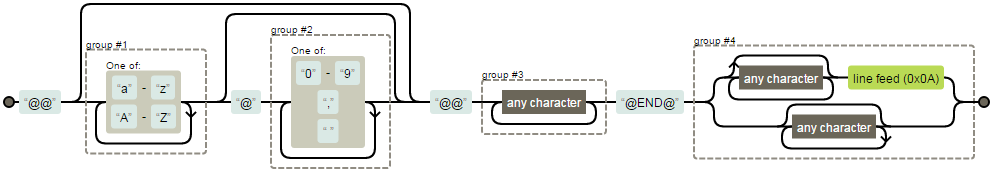
\includegraphics[width=1\textwidth]{rys/implementacja/regex.png}
    \caption{Graf przedstawiający wzorzec przechwytujący informacje o selekcji w szablonach}
    \label{fig:Wzorzec}
\end{figure}
\par
Grupy przechwytujące:
\begin{itemize}
\item Grupa 1: Nazwa środowiska
\item Grupa 2: Grupowanie
\item Grupa 3: Zapytanie SQL
\item Grupa 4: Przechwycenie pozostałości (wykorzystane tylko w celu znalezienia końca informacji)
\end{itemize}
\vspace{5mm}
 \par
W języku JAVA zaimplementowana została już obsługa wyrażeń regularnych. Wystarczy więc wykorzystać dostępne klasy \texttt{Pattern} oraz \texttt{Matcher}. Przez wywołanie statycznej metody \texttt{compile} z flagami \texttt{Pattern.DOTALL | Pattern.MULTILINE} uzyskamy odpowiednio skompilowane wyrażenie regularne. Zewnętrzna pętla wykorzystana będzie do iterowania szablonów, natomiast wewnętrzna pętla do zapisu znalezionych selekcji dla danego szablonu. Składowa \texttt{sqlinfo} po jednorazowym wywołaniu tej metody przechowywać będzie dla k-tego szablonu wszystkie znalezione selekcje.

 \begin{lstlisting}[numbers=left,firstnumber=214]
public void parseSqlStatements(String pat)
{

 if(pat.equals(""))
  pat = "@@(?:([a-zA-Z]+)(?:@([0-9, ]+))?)?@@(.+?)@END@(.*?\\n|.*)";
    
 Pattern localPattern = Pattern.compile(pat, Pattern.DOTALL | Pattern.MULTILINE);
 Matcher localMatcher;
 for(int k=0;k < this.getLenght();k++){

  localMatcher = localPattern.matcher(this.data[k]);
  while (localMatcher.find())
  {
    sqlinfo.get(k).add(new ParsedSQLInfo(localMatcher.group(3),
    localMatcher.group(1), localMatcher.group(2), localMatcher.end()));
   }
  }
}
  \end{lstlisting}
   
\subsubsection*{Metoda sprawdzająca zdolność szablonu do kompilacji}

W czasie tworzenia projektu wynikła potrzeba wprowadzenia dodatkowej funkcji, która wykorzystywana jest w klasie odpowiadającej za kompilacje szablonów. Poniższa metoda sprawdza każdy szablon czy jest możliwe skompilowanie go, poprzez weryfikację czy wewnątrz szablonu znajduje się początek i koniec środowiska \texttt{document}. Informacje te zapisywane są odpowiednie dla k-tego szablonu w składowej klasy, która jest tablicą. Dla kompilowalnych szablonów zapisywana jest odpowiednio jedynka, natomiast dla braku możliwości kompilacji jest to zero. Wywoływana jest ona w metodzie ładowania szablonu(138 linia).

 \begin{lstlisting}[numbers=left,firstnumber=155]
 private void isCompilable(int k) {
  String start = "\\begin{document}";
  String end = "\\end{document}";
  int from = data[k].indexOf(start);
  int to = data[k].indexOf(end);
        
  if(from == -1 || to == -1)
   compileable[k] = 0;
  else
   compileable[k] = 1;
 }
  \end{lstlisting}
  
\subsection{Metody prostego przetwarzania danych z bazy}

Podsekcja opisuje proces przetwarzania danych pobranych z bazy danych do formatu, który jest w stanie odczytać kompilator LaTeX.

\subsubsection*{Metoda przygotowująca dane i wybierająca rodzaj przetwarzania}

Do metody przekazywane są następujące parametry:
\begin{itemize}
\item \texttt{int k} - Indeks pliku zapisanego w składowej
\item \texttt{int c} - Indeks selekcji ze znalezionych w danym pliku
\item\texttt{String  env} - Znaleziona nazwa środowiska dla danej selekcji
\item \texttt{String  grouping} - Znaleziona informacja o grupowaniu danych
\item \texttt{RecordSet rs} - Dane pobrane z bazy danych
\end{itemize}
\vspace{5mm}
Jeśli parametr \texttt{env} jest pusty wygenerowana zostanie nazwa środowiska za pomocą nazwy pliku oraz dodany do tego postfiks, który będzie dużą literą alfabetu łacińskiego w zależności od numeru selekcji. 
\par
Jeśli parametr \texttt{grouping} jest pusty to znaczy ze wykorzystane zostanie proste przetwarzanie poprzez wywołanie metody \texttt{prepareValuesSimple(k,c, prefix, rs);}.
\par
 W przeciwnym wypadku przygotowana zostanie tablica \texttt{int group}, 
 która zawierająca informację o ilości i wielkości wszystkich grup. Tablica ta zostanie przekazana przy wywołaniu metody, która
 przetwarza grupowanie danych \texttt{prepareValuesGrouping(group, 0,0,rs.get\_rows(),  rs, prefix)}. Metoda ta potrzebuje pewnych inicjacji w postaci parametrów 0, dlatego że jest to metoda rekurencyjna. Dokładny opis znajduje się w późniejszej sekcji.
 
 \begin{lstlisting}[numbers=left,firstnumber=246]
public int prepareValues(int k,int c,String env,String grouping,RecordSet rs){
 if(rs == null)
   return(0);

  char l = (char) ('A' + (char)c);
  String prefix;
  if(env == null)
   prefix =  listOfFiles[k].getName().substring(0,
	   listOfFiles[k].getName().indexOf('.')) + l;
  else
   prefix = env;
      
  if(grouping == null){
   prepareValuesSimple(k,c, prefix, rs);
   System.out.println(  rs.get_rows() + " records SQL" + (c+1));  
  }
  else{
   String[] groupstmp = grouping.split(",");
   int[] group = new int[groupstmp.length];
   for(int i=0;i<groupstmp.length;i++)
    group[i] = Integer.parseInt(groupstmp[i]);
           
   sqlinfo.get(k).get(c).setData(prepareValuesGrouping(
	   group, 0,0,rs.get_rows(),  rs, prefix)); 
          
   groupstmp = null;
   group = null;
   System.out.println(  rs.get_rows() + " records SQL" + (c+1));   
   rs = null;
   }
  return(0);  
 }
  \end{lstlisting}


\subsubsection*{Metoda prostego przetworzenia danych}

%bib Java. Kompendium programisty. Wydanie VIII
Metoda ma na celu utworzenie dla każdego przekazanego rekordu w parametrze metody \texttt{RecordSet rs } utworzenie linii tekstu zawierającego wywołanie środowiska o nazwie przekazanej w parametrze metody \texttt{String prefix} i od parametrów, którymi będą kolejne pola w rekordach. 
\par 
Obiekt typu \texttt{RecordSet} jest macierzą typu \texttt{String}, którą należy połączyć w odpowiedni sposób. Do tego celu wykorzystana została klasa \texttt{StringBuilder}, która potrafi połączyć znaczą ilość obiektów typu \texttt{String} w optymalny sposób poprzez metodę \texttt{append} i utworzyć z nich jeden obiekt.
\par
W odpowiedni sposób przygotowane dane zapisane zostają pod  \texttt{sqlinfo.get(k).get(c).setData(temp2); } czyli k-tym plikiem oraz c-tym zapytaniem w składowej do tego przeznaczonej.

 \begin{lstlisting}[numbers=left,firstnumber=289]
 public int prepareValuesSimple(int k,int c, String prefix, RecordSet rs){
  String temp1 = "";
  String temp2 = "";

  StringBuilder result = new StringBuilder(); 
       
  for(int i=0; i < rs.get_rows(); i++){
   temp1 = "\\" + prefix;
   for(int j=0; j < rs.get_cols(); j++)
    temp1 += "{" + rs.getVal(i, j) + "}";
        
   result.append(temp1 + "\n");
  }

  temp2 = result.toString();
  sqlinfo.get(k).get(c).setData(temp2); 
  return(0);
}
  \end{lstlisting}

\subsection{Metody grupujące dane z bazy}

Do stworzenia drzewa grup, opisanego w sekcji działania algorytmu zaimplementowana została specjalnie do tego celu rekurencyjna metoda, która wywołuje samą siebie. Ze względu na czytelność, podzielona została ona na 2 metody opisane poniżej.

\subsubsection*{Metoda rekurencyjnie generująca grupy}

Metoda przyjmuje parametry:
\begin{itemize}
\item \texttt{int[] group} - tablica grup
\item \texttt{int gid} - Indeks aktualnej grupy
\item\texttt{int s} - Numer rekordu od którego rozpoczyna pracę w tym wywołaniu w \texttt{rs record}
\item \texttt{int e} - Numer rekordu na którym kończy pracę w tym wywołaniu w \texttt{rs record}
\item \texttt{RecordSet rs} - Dane pobrane z bazy danych
\item \texttt{String prefix} - Nazwa środowiska
\end{itemize}
\vspace{5mm}
Dla aktualnej grupy i zakresu działania metoda uruchamia proste przetwarzanie danych lub w razie istnienia niższych grup, wykonuje kolejny podział na kolejną grupę poprzez analizę zawartości pól po których jest ta grupa. Dla każdej unikatowej kombinacji tworzone jest wywołanie grupy z tymi wartościami, a następnie metoda wywołuje samą siebie od zakresu w którym występują dane o unikatowych wartościach. Wywołanie w ten sposób tej metody zwróci zawartość tej grupy, która zostanie umiejscowiona pomiędzy wywołaniem grupy (startu) oraz wywołaniem zamknięcia grupy (końca).
\par 
Do nazwy grupy zgodnie z algorytmem dodawane są litery alfabetu łacińskiego w zależności od numeru poziomu grupy.
\par
Jeśli skończą się niższe grupy do utworzenia w czasie działania metody na danym zakresie danych, wywoływana jest metoda \texttt{prepareInjectValues(prefix, rs,s,e,sc)} która zwróci dla danego zakresu rekordów i wyciętych odpowiednich pól, proste wywołania środowiska o przekazanej nazwie. Wywołanie tej metody, zwróci przetworzone odpowiednio wartości, które przekazane zostaną dalej do grupy z której została wywołana metoda grupująca.

 \begin{lstlisting}[numbers=left,firstnumber=322]
 public String prepareValuesGrouping(
	 int[] group, int gid,int s, int e, RecordSet rs, String prefix){

  if(gid == group.length){
   int sc=0;
   for(int i=0;i<gid;i++)
    sc += group[i];
   return(prepareInjectValues(prefix, rs,s,e,sc));
   }
  if(gid < group.length){
   StringBuilder result = new StringBuilder(); 
   char x;
   String strreturn="";
   String strtmp="";
   String endin;
   int index1=s;
   int index2=s;
   int check=0;

   int col =0;
   for(int i=0;i<gid;i++)
    col += group[i];
          
   index2++;
   while(index2 <= rs.get_rows() && index2 <= e){
    if(index2 == rs.get_rows() || index2 == e)
     check = 2;
    else{
     for(int i=0;i<group[gid];i++)
      if(!rs.getVal(index1,i+col).equals(rs.getVal(index2,i+col)))check = 1;
    }
           
    if(check >= 1){

     x = (char) ('A' + (char)gid);
     strtmp= "\\" + prefix+x;
               
               
     for(int i=0;i<group[gid];i++)
      strtmp += "{" + rs.getVal(index1,i+col)+ "}";
               
     strtmp += "\n"; 
     strtmp += prepareValuesGrouping(group, gid+1,index1, index2, rs, prefix);
     endin =  "\\end" + prefix + x + "\n";

     result.append(strtmp.concat(endin));

     index1 = index2;
     check = 0;
    }
    index2++;
   }
  return(result.toString());    
  }
return("");
}
\end{lstlisting}


\subsubsection*{Metoda przetwarzająca dane po zgrupowaniu}


Metoda prostego już przetwarzania danych rozszerzona o dodatkowe rozróżnianie rekordów oraz pól, które ma zapisywać. 
\par 
W parametrach przekazywane są informacje:
\begin{itemize}
\item \texttt{int s} - rekord od którego rozpoczyna pracę w \texttt{rs record}
\item \texttt{int c} - rekord na którym kończy pracę w \texttt{rs record}
\item \texttt{int sc} - numer pole w rekordzie od którego ma dopiero pobierać dane, a wszystkie wcześniejsze pominąć
\item\texttt{String  prefix} -  nazwa środowiska dla danej selekcji
\item \texttt{RecordSet rs} - Dane pobrane z bazy danych
\end{itemize}
\vspace{5mm}
Metoda ostatecznie zwraca przetworzone dane. Łączenie tych danych w całość odbędzie się w metodzie \texttt{ prepareValuesGrouping} opisanej wcześniej.

 \begin{lstlisting}[numbers=left,firstnumber=380]
 private String prepareInjectValues(String prefix,RecordSet rs,int s, int e,int sc){
  String temp1 = "";
  String temp2 = "";

  StringBuilder result = new StringBuilder();

  for(int i=s; i < e; i++){
   temp1 = "\\" + prefix;
   for(int j=sc; j < rs.get_cols(); j++)
    temp1 += "{" + rs.getVal(i, j) + "}";

   temp1 += "\n";
   result.append(temp1);

      }

  return(result.toString());
}    
\end{lstlisting}


\subsection{Metoda uzupełnienia szablonu o przetworzone dane}

Metoda dodająca przetworzone wartości do zmiennej przechowującej zawartość szablonu. Dodawanie odbywa się od ostatniego zapytania do pierwszego, aby nie zmieniać dodatkowo zapamiętanych indeksów miejsc, w których znajdują się selekcje.

 \begin{lstlisting}[numbers=left,firstnumber=402]
 public void InjectValues(int k){
  int to;
  for(int i=sqlinfo.get(k).size()-1; i >= 0; i--){
    to = sqlinfo.get(k).get(i).getIndex();
    data[k] = data[k].substring(0,to) + sqlinfo.get(k).get(i).getData() 
    + data[k].substring(to,data[k].length());
   }
        
 }
\end{lstlisting}


\subsection{Akcesory}
Akcesory (gettery i settery) to określenie metod jakie wykorzystuje obiekt do pobrania wartości i modyfikacji swoich atrybutów. Są one bardzo często dołączane do klas przez programistów Javy i nawet niektóre edytory (np. Eclipse) posiadają funkcjonalność automatycznego wygenerowania ich. Poniżej przedstawiony został każdy akcesor do klasy z krótką informacją co pobiera:
\par
\begin{itemize}

\item Pobranie ilości szablonów:
 \begin{lstlisting}[numbers=left,firstnumber=414]
 public int getLenght(){return data.length;}
 \end{lstlisting}
 
\item Pobranie ścieżki do pliku uzupełnionego szablonu w tex:
 \begin{lstlisting}[numbers=left,firstnumber=419]
 public String getSavedPath(int k){return (pathoutput + listOfFiles[k].getName());}
     \end{lstlisting}
     
\item Pobranie ścieżki wynikowej:
 \begin{lstlisting}[numbers=left,firstnumber=423]
 public String getOutputPath(){return (pathoutput);}
     \end{lstlisting}
     
\item Pobranie informacji o tym czy k-ty szablon może zostać skompilowany:
 \begin{lstlisting}[numbers=left,firstnumber=429]
 public int compileCheck(int k){return(compileable[k]);}
     \end{lstlisting}
\item Pobranie wszystkich informacji o selekcji dla k-tego szablonu:
 \begin{lstlisting}[numbers=left,firstnumber=436]
 public ArrayList<ParsedSQLInfo> getStmts(int k){return sqlinfo.get(k);}
     \end{lstlisting}
\item Pobranie nazwy pliku o indeksie k: 
 \begin{lstlisting}[numbers=left,firstnumber=443]
 public String getFileName(int k ){ return(listOfFiles[k].getName());}
     \end{lstlisting}

\end{itemize}

\section{Zarządzanie kompilatorem LaTeX - klasa LatexCompiler}

Uzupełnione szablony przez klasę Templates, należy następnie skompilować przy pomocy wywołania kompilatora który został podany w konfiguracji.
Do tego posłuży właśnie klasa LatexCompiler, która wywoła polecenie w konsoli systemowej, uruchamiające kompilator od odpowiednich parametrów.
W składowych zapamiętane zostaną informacje o ścieżce do kompilatora oraz ścieżka plików wynikowych.

 \begin{lstlisting}[numbers=left,firstnumber=18]
public class LatexCompiler {
    
 String latexcompilerpath;
 String pdfoutput;
\end{lstlisting}

\subsubsection*{Konstruktor}
Konstruktor z 2 parametrami przekazującymi ścieżkę do kompilatora oraz katalog wynikowy, będzie miał za zadanie zapisać te parametry do składowych oraz sprawdzić czy katalog wynikowy istnieje. W razie jego braku, utworzy go.

 \begin{lstlisting}[numbers=left,firstnumber=31]
public LatexCompiler(String latexcompilerpathh,String pdfoutputt){
 latexcompilerpath = latexcompilerpathh;
 pdfoutput = pdfoutputt;

 File tmp = new File(pdfoutput);
 if (!tmp.exists()) {
  tmp.mkdirs();
 }
    
 }
\end{lstlisting}

\subsubsection*{Metoda wywołująca kompilacje pliku LaTeX}

Parametrem metody jest nazwa pliku, który zostanie poddany kompilacji.  Następnie aby skompilować dany plik należy uruchomić kompilator, do którego ścieżka zapisana jest w składowej \texttt{latexcompilerpath} z parametrem \texttt{--output-directory} w którym przekażemy katalog wynikowy oraz z parametrem którym jest ścieżka pliku do kompilacji. Wygenerowane polecenie zostanie wywołane w powłoce systemowej za pomocą metody \texttt{executeCommand} opisanej w podsekcji niżej.

 \begin{lstlisting}[numbers=left,firstnumber=46]
public int compileTemplate(String filetexpath){
 System.out.print( executeCommand(latexcompilerpath
  + " --output-directory=" + pdfoutput + " " + filetexpath));
 return(0);
 }
\end{lstlisting}

\subsubsection*{Metoda wywołująca polecenie powłoki systemu}


Metoda ta ma na celu uruchomić nowy proces, którym będzie wywołanie komendy powłoki przesłanej przez parametr \texttt{String commmand}. \texttt{Runtime.getRuntime().exec("cmd /c start" + command);} Wywoła polecenie w nowym oknie i przypnie proces do zmiennej \texttt{Process p}. Następnie aby synchronicznie wywoływać polecenie jedno po drugim, program czeka na zakończenie procesu. 

 \begin{lstlisting}[numbers=left,firstnumber=56]
private String executeCommand(String command) {
 
 StringBuffer output = new StringBuffer();
 System.out.print("Executing shell command: \n" + "cmd /c start " + command);
 Process p;
 try {
  p = Runtime.getRuntime().exec("cmd /c start " + command);
  p.waitFor();

\end{lstlisting}

\section{Metoda main() - klasa DBRaportLatex }

Metoda \texttt{main()} jest metodą od której program rozpoczyna swoją pracę. Poniżej przedstawione zostaną jej części:

\begin{itemize}

\item Przyjmuje ona argumenty, które można przekazać podczas uruchomienia programu w postaci tablicy Stringów.

 \begin{lstlisting}[numbers=left,firstnumber=38]
public static void main(String[] args) {
\end{lstlisting}
\vspace{5mm}

\item Pierwszą rzeczą którą należy zrobić po uruchomieniu programu jest załadowanie pliku konfiguracyjnego. Dodatkową opcją jest przekazanie nazwy pliku konfiguracyjnego jako pierwszy argument. Ładowanie konfiguracja odbywa się poprzez stworzenie nowego obiektu klasy \texttt{Config} przez wywołanie konstruktora z 1 parametrem, a dokładniej nazwą pliku konfiguracyjnego:

 \begin{lstlisting}[numbers=left,firstnumber=44]
 Config cfg;
        
 if(args.length == 0)
  cfg = new Config("dblatexraportconfig.bat");
 else{
  System.out.print(args[0] + "\n");
  cfg = new Config(args[0]);
 }
\end{lstlisting}
\vspace{5mm}

\item Kolejną rzeczą do zrobienia jest uzyskanie połączenia z bazą danych. Wykorzystane zostaną przy tym zmienne załadowane z pliku konfiguracyjnego poprzez wywołanie metody \texttt{getString} na obiekcie \texttt{cfg}. Do stworzenia połączenia wykorzystany zostanie obiekt klasy \texttt{DBHandle}. Po utworzeniu obiektu przez konstruktor sparametryzowany do przekazane zostaną odpowiednie zmienne konfiguracyjne, połączenie powinno zostać utworzone:


 \begin{lstlisting}[numbers=left,firstnumber=61]
 DBHandle FBH = new DBHandle(cfg.getString("dbengine"),cfg.getString("hostname"),
  cfg.getString("port"), cfg.getString("dbpath"),
  cfg.getString("dbencoding"), cfg.getString("user"),
  cfg.getString("password"));
\end{lstlisting}
\vspace{5mm}
\item Inicjalizacja obiektu zarządzającego kompilacją:

 \begin{lstlisting}[numbers=left,firstnumber=67]
 LatexCompiler comp = new LatexCompiler(cfg.getString("pdflatexpath"),
 cfg.getString("output"));
\end{lstlisting}

\vspace{5mm}
\item Inicjalizacja obiektu zarządzającego szablonami:

 \begin{lstlisting}[numbers=left,firstnumber=72]
 Templates temps = new Templates(cfg.getString("templatepath"),
  cfg.getString("output"), cfg.getString("encodingtex"));
\end{lstlisting}

\vspace{5mm}
\item Załadowanie wszystkich szablonów do pamięci za pomocą metody \texttt{loadAllTemplates();} na zainicjalizowanym odpowiednimi zmiennymi, obiekcie zarządzającym szablonami:

 \begin{lstlisting}[numbers=left,firstnumber=85]
 temps.loadAllTemplates();
\end{lstlisting}

\vspace{5mm}
\item Przygotowanie zmiennych potrzebnych do parsowania szablonów oraz wywołanie metody parsującej wszystkie szablony od wyrażenia regularnego zapisanego w pliku konfiguracyjnym (jeśli nie zostało wpisane wyrażenie regularne, użyte zostanie standardowe).

 \begin{lstlisting}[numbers=left,firstnumber=91]
 String pattern;
 pattern = cfg.getString("pattern");
 ArrayList<ParsedSQLInfo>  SQLSt;

 temps.parseSqlStatements(pattern);
\end{lstlisting}

\item Główna pętla przechodząca przez wszystkie szablony, pobierająca wszystkie polecenia selekcji z każdego szablonu. Następnie wewnętrzna pętla dla każdego polecenia wywołuje zapytanie w bazie danych i od zwróconych wyników wywołuje funkcje generującą dane do uzupełnienia w szablonie. Na koniec zewnętrznej pętli wywołanie metody uzupełniającej szablon o wygenerowane dane:

 \begin{lstlisting}[numbers=left,firstnumber=98]
 for(int i=0; i < temps.getLenght(); i++){
  System.out.print("\n");
  SQLSt = temps.getStmts(i);
      
  if(SQLSt != null){
   System.out.println(temps.getFileName(i) + " - processing SQL statements");
   for(int j=0; j < SQLSt.size(); j++){

                
    if(SQLSt.get(j).getName() == null){
     System.out.println("no returns SQL" + (j+1)); 
                 
     FBH.executeSQL2(SQLSt.get(j).getQuery());
                
     }
     else
                  
      temps.prepareValues(i,j,SQLSt.get(j).getName(),
      SQLSt.get(j).getGroup(),FBH.executeSQL2(SQLSt.get(j).getQuery()));
    }
   }
 temps.InjectValues(i);
 SQLSt = null;
 } 
\end{lstlisting}


\vspace{5mm}
\item Zapisanie wszystkich uzupełnionych szablonów do plików:

 \begin{lstlisting}[numbers=left,firstnumber=124]
 temps.saveAllTemplates();
\end{lstlisting}
       
\vspace{5mm}
\item Na koniec przeprowadzenie kompilacji uzupełnionych szablonów w zależności od zmiennej \texttt{pdfcompilemainfile} używając przygotowanego obiektu \texttt{comp} klasy \texttt{LatexCompiler}.

       
\begin{lstlisting}[numbers=left,firstnumber=126]
       
 if(cfg.getString("pdfcompilemainfile").equals("ALL"))
  for(int i=0; i < temps.getLenght(); i++){
   comp.compileTemplate(temps.getSavedPath(i));
   }
 if(cfg.getString("pdfcompilemainfile").equals("ONLYBEGDOC"))
  for(int i=0; i < temps.getLenght(); i++){
   if(temps.compileCheck(i)==1)
    comp.compileTemplate(temps.getSavedPath(i));
    }
      
 else if(cfg.getString("pdfcompilemainfile").equals("NONE"));
 else{
          
  String[] tmpfiles = cfg.getString("pdfcompilemainfile").split(",");
          
  for(int i=0;i < tmpfiles.length; i++)
    comp.compileTemplate(temps.getOutputPath() + tmpfiles[i].trim());
  
 }
\end{lstlisting}

\end{itemize}
\section{Kompilacja programu}

Do kompilacji programu dołączony jest plik \emph{build.xml}. Opisuje on przebieg pakowania pliku jar. Ze względu na wykorzystanie paru zewnętrznych bibliotek, tworzony był katalog \emph{library} zawierający te biblioteki i aby tego uniknąć zastosowana została funkcja pakująca wszystkie biblioteki do jednego pliku jar. W listingu poniżej pokazana jest konfiguracja pliku \emph{build.xml}:

 \begin{lstlisting}
 <?xml version="1.0" encoding="UTF-8"?>

<project name="DBRaportLatex" default="default" basedir=".">
    <description>Builds, tests, and runs the project DBRaportLatex.</description>
    <import file="nbproject/build-impl.xml"/>
<target name="-post-jar">

    <property name="store.jar.name" value="DBRaportLatex"/>

    <property name="store.dir" value="dist"/>
    <property name="store.jar" value="${store.dir}/${store.jar.name}.jar"/>

    <echo message="Packaging ${application.title} into a single JAR at ${store.jar}"/>

    <jar destfile="${store.dir}/temp_final.jar" filesetmanifest="skip">
        <zipgroupfileset dir="dist" includes="*.jar"/>
        <zipgroupfileset dir="dist/lib" includes="*.jar"/>

        <manifest>
            <attribute name="Main-Class" value="${main.class}"/>
        </manifest>
    </jar>

    <zip destfile="${store.jar}">
        <zipfileset src="${store.dir}/temp_final.jar"
        excludes="META-INF/*.SF, META-INF/*.DSA, META-INF/*.RSA"/>
    </zip>

    <delete file="${store.dir}/temp_final.jar"/>
    <delete dir="${store.dir}/lib"/>
    <delete file="${store.dir}/README.TXT"/>
</target>
  
</project>
\end{lstlisting}



\chapter{Uruchomienie oraz testowanie systemu}
Przed wdrożeniem programu do realnego systemu, program należy przetestować. Testy powinny być prowadzone na bazie danych która jest odwzorowaniem istniejącej już bazy, ponieważ idea testów jest taka, że po podmianie bazy danych na realną wszystko ma działać bez zmian. Jedyną różnicą może tylko zapis połączenia w pliku konfiguracyjnym. Do przeprowadzenia testów potrzebne więc będzie odtworzenie przyszłego środowiska, w którym będzie działać program, przygotować szablony dokumentów, które są wytwarzane w procesie rekrutacji oraz wygenerować dokumenty. Ostatnim już krokiem będzie sprawdzenie czy podczas tego procesu nie ma żadnych komplikacji oraz czy wygenerowane dokumenty nie zawierają błędów.
\section{Wstępne ustalenia}

Przed rozpoczęciem jakichkolwiek działań należy przygotować podstawowe rzeczy do rozpoczęcia testów.

\subsection{Specyfikacja maszyny do testów}
Testy przeprowadzone będą na komputerze o następującej specyfikacji:
\begin{lstlisting}
OS Name	Microsoft Windows 7 Ultimate
Version	6.1.7601 Service Pack 1 Build 7601
System Model	Z97-lstlisting
System Type	x64-based PC
Processor	Intel(R) Core(TM) i5-4590 CPU @ 3.30GHz,
3301 Mhz, 4 Core(s), 4 Logical Processor(s)
Installed Physical Memory (RAM)	8,00 GB
Total Physical Memory	7,86 GB
Available Physical Memory	3,99 GB
Total Virtual Memory	9,86 GB
Available Virtual Memory	3,75 GB
Page File Space	2,00 GB
\end{lstlisting}

Do działania programu \emph{DBRaportlatex} zainstalowana została JAVA w wersji:
\begin{lstlisting}
C:\Users\Pawlos>java -version
java version "1.8.0_60"
Java(TM) SE Runtime Environment (build 1.8.0_60-b27)
Java HotSpot(TM) 64-Bit Server VM (build 25.60-b23, mixed mode)
\end{lstlisting}

\subsection{Struktura katalogowa}

Do przejrzystego przechowywania wszystkich rzeczy potrzebnych w systemie rekrutacji, potrzebna będzie odpowiednia struktura katalogów. Do przechowywania potrzebne będą: \\
\begin{itemize}
\item program: \texttt{DBLatexRaport.jar}
\item plik konfiguracyjny: \texttt{dblatexraportconfig.bat}
\item środowisko kompilacji latex
\item szablony dokumentów 
\item plik bazy danych(tylko w testach)
\item pliki wynikowe
\item biblioteki potrzebne dla silnika bazy danych firebird w wersji embedded \\
\end{itemize}

Proponowana struktura więc może wyglądać następująco:

%\dirtree{%
 %.1 /.
 %.2 Firebird.
 %.2 output.
 %.2 template.
 %.2 texlive.
 %.2 DBLatexRaport.jar.
 %.2 dblatexraportconfig.bat.
 %.2 rekrutacja.fdb.
%}
\vspace{5mm}
Do katalogu \emph{texlive} przegrane zostało środowisko do kompilacji plików latex. W katalogu firebird są biblioteki tylko na czas testów do wersji embedded bazy danych. W katalogu \emph{template} zapisane zostaną szablony dokumentów.


\section{Generowanie przykładowych danych}

W celu przetestowania systemu generowania raportów w procesie rekrutacji kandydatów na studia potrzebne będą testowe dane w dokładnie tej samej strukturze, co w systemie rekrutacji, ze względu na fakt, iż w szablonach LaTeX znajdują się zapytania SQL do tabel w znajdujących się w bazie danych. 
W celu otrzymania tych danych potrzebne będzie:
\begin{enumerate}

\item	Utworzenie nowej bazy danych na silniku Firebird’a 
\item	Stworzenie struktury tabel odzwierciedlającą strukturę w systemie uczelnianym.
\item	Wygenerowanie wyczerpującej potrzeby testu ilości testowych danych osobowych.
\item	Uzupełnienie tabel danymi, które zostały wygenerowane wcześniej oraz dodanie do nich dodatkowych, jednocześnie losowych, informacji na temat procesu rekrutacji.
\vspace{5mm}
\end{enumerate}
Po wykonaniu tych kroków, powinna powstać baza danych do której bez problem program połączy się i uzyska z niej potrzebne dane dokładnie w ten sam sposób jak z realnej bazy danych.

\subsection{ Tworzenie bazy danych }

Do stworzenia pliku bazy danych na silniku firebird’a posłużyć się można narzędziem dostępnym w katalogu bin zainstalowanego serwera firebird.  Narzędzie to pozwala z linii komend tworzyć i łączyć się z bazami danych. W tym przypadku użyta zostanie komenda \texttt{CREATE DATABASE}
\begin{lstlisting}
C:\Program Files\Firebird\bin>isql
SQL>CREATE DATABASE 'D:\test systemu\rekrutacja.fdb'
CON>user 'SYSDBA' password 'masterkey';
\end{lstlisting}
Po wykonaniu tego polecenia zostanie utworzona baza danych. Takie same dane należy teraz wpisać do pliku konfiguracyjnego programu czyli \texttt{DBLatexRaport.bat} aby program mógł się połączyć z tą bazą:
\begin{lstlisting}
dbengine=firebirdsql
hostname=//localhost
port=3050
dbpath=D:\test systemu\rekrutacja.fdb
user=SYSDBA
password= masterkey
\end{lstlisting}
\subsection{ Stworzenie struktury bazy}

Dotychczasowy system wykorzystywał tabelę (widok) która była generowana dynamicznie i która zawiera wszystkich kandydatów w rekrutacji. Zawiera ona wszystkie dane potrzebne do wytworzenia dokumentów. Jeden rekord to jeden student ze wszystkimi informacjami na jego temat. Dodatkowo jeszcze potrzebna jest tabela z informacjami na temat rekrutacji, takimi jak na przykład nazwisko i imię przewodniczącego komisji, czy data wydania decyzji przyjęcia studenta. Z tych tabel będą pobierane informacje, natomiast do wygenerowania danych potrzebne będą dwie dodatkowe tymczasowe tabele.
Tabela główna z kandydatami(zapis SQL):
\begin{lstlisting}
CREATE TABLE KANDYDAT_ALIGEZA (
    STUD_ID                        INTEGER NOT NULL,
    OSOBA_ID                       INTEGER NOT NULL,
    STUD_NRTECZKI                  INTEGER,
    NAZWISKO                       VARCHAR(100),
    IMIE                           VARCHAR(100),
    NAZWISKOIMIONA                 VARCHAR(200),
    ADR_ULICA_MIEJSCOWOSC_NR_DOMU  VARCHAR(200),
    ADR_KOD_POCZTOWY_POCZTA        VARCHAR(100),
    STUDIA_NAZWA                   VARCHAR(100),
    STUD_ILPUNKTOW                 INTEGER,
    STUD_ILPUNKTOWKREM             INTEGER,
    TOKNAUKI_NAZWATOKU             VARCHAR(200),
    KIERUNEK                       VARCHAR(100),
    SPEC_ID                        INTEGER,
    DATAPRZYJECIAPODANIA           DATE,
    TOKNAUKI_ID                    INTEGER,
    OSOBA_PESEL                    VARCHAR(50),
    KIERUNEK_MY                    VARCHAR(200),
    FORMA_STUDIOW_MY               VARCHAR(200),
    STOPIEN_STUDIOW_MY             VARCHAR(100),
    KIERUNEK_FORMA_SKROT_MY        VARCHAR(100),
    NR_DECYZJI                     VARCHAR(100),
    CZY_PRZYJETY                   INTEGER,
    DATA_DECYZJI                   DATE,
    ILE_PUNKTOW                    INTEGER,
    PANPANI                        CHAR(1)
);
\end{lstlisting}
Tabela z dodatkowymi informacjami(wartości przypisane są do kluczy tekstowych, jest to tablica asocjacyjna):
\begin{lstlisting}
CREATE TABLE SETUP_ALIGEZA (
    KLUCZ    VARCHAR(50) NOT NULL,
    WARTOSC  VARCHAR(100)
);
\end{lstlisting}
Tymczasowa tabela do zaimportowania listy imion i nazwisk oraz losowych peseli.
\begin{lstlisting}
CREATE TABLE DANE (
    IMIE_NAZ  VARCHAR(200),
    ADRES     VARCHAR(200),
    PESEL     VARCHAR(50),
    NAZWISKO  VARCHAR(100),
    IMIE      VARCHAR(100)
);
\end{lstlisting}
Tymczasowa tabela do procedury losowego uzupełniania informacji o rekrucie o kierunku jaki wybrał.
\begin{lstlisting}
CREATE TABLE TOKNAUKI_ALIGEZA (
    TOKNAUKI_ID              INTEGER NOT NULL,
    KIERUNEK_MY              VARCHAR(50),
    FORMA_STUDIOW_MY         VARCHAR(50),
    STOPIEN_STUDIOW_MY       VARCHAR(50),
    KIERUNEK_FORMA_SKROT_MY  VARCHAR(10),
    LICZBA_MIEJSC            SMALLINT,
    DATA_DECYZJI_OD          TIMESTAMP,
    DATA_DECYZJI_DO          TIMESTAMP,
    KOD_IKR                  VARCHAR(3)
);
\end{lstlisting}
\subsection{ Generowanie testowych danych osobowych}

Do wygenerowania kandydatów potrzebne jest imię, nazwisko oraz adres. Takie dane dostępne są w książkach telefonicznych. Posługując się jedną z nich stworzony został plik \emph{CSV} o separatorze „;” zawierający po kolei imię z nazwiskiem, adres, pesel, nazwisko oraz imię. Pesel został dodany do każdej osoby jako losowy ciąg cyfr spełniający walidację peselu. Ze względu na fakt iż pesel został wygenerowany losowo,  w wygenerowanych dokumentach nie będzie poprawnie przypisana płeć do imienia. Dlatego tylko do testów ustawione zostanie 5 pierwszych kandydatów jako płeć żeńska, a cała reszta męska.\\
Struktura pliku:
\begin{lstlisting}
 Abram Andrzej; Lwowska 116;88071640299;Abram;Andrzej
 Abram Halina; Ludwika Zamenhofa 2;86111210691;Abram;Halina
...

\end{lstlisting}

Tak sformatowany plik \emph{CSV},  łatwo zaimportować do bazy danych do tabeli \texttt{dane} ze względu na identyczną kolejność danych w kolumnach. Do importu wykorzystana została funkcja programu \emph{IBExpert}, \texttt{import data}. Jedna linijka w pliku zostaje zaimportowana jako jeden rekord, w którym każde pole po kolei odpowiada wartościom między średnikami. Zaimportowanych w ten sposób zostało 10001 rekordów (osób) do tabeli \texttt{dane} do dalszych manipulacji, co całkowicie wyczerpuje ilość kandydatów potrzebnych do testów. Ze statystyk wynika, że na uczelni średnio na rekrutacje przypada około trzystu kandydatów.

\subsection{Generowanie kandydatów na studentów}

Kolejnym krokiem jest uzupełnienie tabeli z tokami studiów. W testach dodanych zostało 8 przykładowych toków nauki. 

\begin{lstlisting}
1 Informatyka	niestacjonarne	pierwszego stopnia	INF-n				
2 Mechatronika	niestacjonarne	pierwszego stopnia	MT-n				
3 Mechatronika	stacjonarne	pierwszego stopnia	MT-s				
...
\end{lstlisting}
Uzupełnienia wymaga także tabela z dodatkowymi informacjami \texttt{setup\_aligeza} przykładowymi danymi:
\begin{lstlisting}
dataWydaniaDecyzji	09.10.2015
miejsceWydaniaDecyzji	Nowy Sącz
przewodniczacyIKR	mgr inż. Sławomir Jurkowski
rokAkademicki	2015/2016
czyUwzglednicDateWydaniaDecyzji	N
...

\end{lstlisting}

Mając już to wszystko potrzebna jest procedura, która utworzy listę kandydatów z tych wszystkich danych. 

\begin{lstlisting}
create procedure GENERUJ
returns (
    TESTCHAR varchar(50),
    TEST integer)
as
declare variable IMIE varchar(100);
declare variable NAZ varchar(100);
declare variable IMIENAZ varchar(200);
declare variable ADRES varchar(200);
declare variable PESEL varchar(50);
declare variable LICZNIK integer;
declare variable STOPIEN varchar(50);
declare variable KIERUNEK varchar(50);
declare variable FORMA varchar(50);
declare variable SKROT varchar(10);
declare variable RANDINT integer;
declare variable PUNKTY integer;
declare variable CZY_PRZYJETY integer;
declare variable DATA_DEC varchar(100);
begin
licznik = 1;
for select * from dane into
:imienaz,:adres,:pesel,:naz,:imie
do
begin
randint = CAST(round(rand()*7+1) as INTEGER);
punkty = CAST(round(rand()*500) as INTEGER);
if(punkty > 250) then czy_przyjety = 1;
if(punkty <= 250) then czy_przyjety = 2;

select kierunek_my,forma_studiow_my,stopien_studiow_my,
kierunek_forma_skrot_my
FROM toknauki_aligeza where toknauki_id = :randint
INTO :kierunek,:forma,:stopien,:skrot;

select wartosc FROM setup_aligeza 
WHERE klucz='dataWydaniaDecyzji'
INTO :data_dec;

INSERT INTO kandydat_aligeza (stud_id,osoba_id,stud_nrteczki,nazwisko,imie,
	nazwiskoimiona,adr_ulica_miejscowosc_nr_domu,adr_kod_pocztowy_poczta,
	osoba_pesel,panpani, studia_nazwa,toknauki_nazwatoku,kierunek, 
	kierunek_my,forma_studiow_my,stopien_studiow_my,
	kierunek_forma_skrot_my,    stud_ilpunktow,stud_ilpunktowkrem,
	ile_punktow,czy_przyjety,data_decyzji,nr_decyzji,dataprzyjeciapodania)
VALUES (:licznik,:licznik,cast(round(rand()*200+1) as integer),
	:naz,:imie,:imienaz,:adres, cast( 'Nowy Sacz 33-300' as varchar(100)),
	:pesel,cast( 'M' as char(1)),    :forma,:kierunek || 
	' N inz. 3.50 2015/2016 zimowy',:kierunek,:kierunek,:forma,
	:stopien,:skrot,    :punkty,:punkty,:punkty,:czy_przyjety,
	cast(:data_dec as DATE),'328/2015','2015-08-14');

licznik = :licznik + 1;
end
test = :licznik;
suspend;
end
\end{lstlisting}
Powyższa procedura z jednej osoby z tabeli \texttt{dane} tworzy jednego kandydata, losując mu tok nauki, ilość punktów oraz czy zostanie przyjęty lub nie. Dodawane są także pewne stałe wartości, podobne do tych w oryginalnej bazie danych, które nie wymagają uzmiennienia. Procedura ta, po jednorazowym wywołaniu, wygenerowała 10001 rekordów w tabeli \texttt{kandydat\_aligeza}. Daje to wystarczającą ilość testowych kandydatów do przeprowadzenia testów. Baza danych z przeprowadzonych testów znajduje się w załączniku.

\section{Dodanie zapytań SQL do szablonów}

Stworzone szablony w poprzednim rozdziale nie zawierają zapytań, które odzwierciedlały by wyselekcjonowanie danych z istniejącej struktury bazy. Zawierają tylko sztywne dane testujące środowiska LaTeX'owe. Aby szablony podczas procesu tworzenia dokumentów zostały uzupełnione poprawnymi danymi potrzeba je uzupełnić o odpowiednia zapytania SQL w odpowiedniej formie tak aby parser zawarty w programie był wstanie je znaleźć i wykonać.
\par 
Potrzebnych jest 9 zapytań, za pomocą których wyciągnięte zostaną dane do szablonów. Poniżej opisane zostały każde z zapytań oraz dla każdego przykład danych jakie zostaną wyselekcjonowane z bazy przez to zapytanie. Ta sekcja skupia się tylko i wyłącznie na uzyskaniu potrzebnych danych do środowisk LaTeX'a, a nie na tym jak one zostaną wykorzystane. Dokładny opis jak wygląda wykorzystanie takiego zapisu znajduje się w rozdziale \ref{ch:szablonyraportowwsystemielatex}. Dodać jeszcze należy ze poniższe zapytania znajdują się pod koniec każdego szablonu, zaraz po zdefiniowaniu środowisk. Takie umiejscowienie tych zapytań sprawi, że dane zostaną uzupełnione zaraz pod tymi zapytaniami.
\par 
\subsubsection*{Szablon z ustawieniami - aaasetup.tex}
Pierwsze zapytanie które zostanie omówione jest to  zapytanie o podstawowe parametry, informacje na temat rekrutacji. Znajduje się ono w pliku \emph{aaasetup.tex}. Plik posiada trzy litery "a" w nazwie, ponieważ program parsujący, otwiera pliki alfabetycznie a zapytanie to, musi zostać wykonane jako pierwsze.  Poniżej mamy przykład danych do zapisania:
 \begin{lstlisting}
\parametrRekrutacyjny{dataWydaniaDecyzji}{09.10.2015}
\parametrRekrutacyjny{miejsceWydaniaDecyzji}{Nowy Sącz}
\parametrRekrutacyjny{rokAkademicki}{2015/2016}
...
\end{lstlisting}
Aby uzyskać takie dane, potrzeba będzie pobrać wszystkie rekordy z tabeli \texttt{setup\_aligeza} (struktura tabeli znajduje się w poprzedniej sekcji) klucz oraz wartość. Zapytanie nie będzie więc zbyt skomplikowane:
 \begin{lstlisting}
SELECT klucz,wartosc FROM setup_aligeza
\end{lstlisting}
Po wywołaniu go, otrzymamy potrzebne nam dane. Jednak aby program parsujący był wstanie znaleźć takie zapytanie w szablonie potrzeba je obudować w odpowiednią konstrukcję, która będzie odpowiadać wyrażeniu regularnemu zapisanemu w parserze. Należy także wpisać nazwę środowiska w odpowiednie miejsce między znakami @@. Dodatkowo należy jeszcze postarać się aby kompilator LaTeX'a zignorował ten zapis i go nie wyświetlał. Do tego celu zastosowana została komenda \texttt{iffalse}.
 \begin{lstlisting}
\iffalse@@parametrRekrutacyjny@@
SELECT klucz,wartosc FROM setup_aligeza
@END@\fi
\end{lstlisting}
\subsubsection*{Szablon protokołu przekazania -  protokolprzekazania.tex}
Następnie zapytanie zawarte w pliku \emph{protokolprzekazania.tex}. Występuje tu nowy problem otworzenia środowiska na początku oraz zamknięcia na końcu. Pokazane jest to na przykładowych danych poniżej:
 \begin{lstlisting}
\protokolprzekazaniaA{1}
\protokolprzekazania{Informatyka ---
 niestacjonarne STUDIA pierwszego stopnia}{1455}
\protokolprzekazania{Informatyka ---
 stacjonarne STUDIA pierwszego stopnia}{729}
\protokolprzekazania{Mechatronika ---
 niestacjonarne STUDIA pierwszego stopnia}{1447}
...
\endprotokolprzekazaniaA        
\end{lstlisting}
\par
Pomijając na razie otwarcie środowiska \texttt{protokolprzekazaniaA\{1\} }oraz zamkniecie \texttt{endprotokolprzekazaniaA}, w zapytaniu potrzebne jest wyświetlić każdy tok nauczania oraz zagregowaną liczbę kandydatów na tym toku. Do agregacji użyte zostanie polecenie \texttt{group} na polu tok by móc otrzymać liczbę kandydatów używając funkcji count(*). Dodatkowo potrzeba także wybrać kandydatów, posiadających daną datę decyzji. Do tego posłuży podzapytanie, które pobierze datę decyzji z aktualnej rekrutacji i porówna ją z datą decyzji dla danego kandydata. 
 \begin{lstlisting}
SELECT  k.kierunek_my||' --- '||k.forma_studiow_my||
' STUDIA '||k.stopien_studiow_my AS tok, count(*) AS ile
FROM kandydat_aligeza k
WHERE  k.data_decyzji=(SELECT wartosc FROM
 setup_aligeza WHERE klucz='dataWydaniaDecyzji') 
GROUP BY tok
\end{lstlisting}
\par
Takie zapytanie wyświetli dane pomiędzy tymi pominiętymi dotychczas komendami. 
Rozwiązaniem wyświetlenia tych komend jest funkcja programu uzupełniającego szablony, a dokładnie funkcja grupowania. Dokładny opis tej funkcji znajduje się w rozdziale \ref{ch:szablonyraportowwsystemielatex}. Do zapytania dodamy jako pierwsze pole wartość 1, a następnie użyta zostanie funkcja grupowania po 1 polu wewnątrz szablonu:
 \begin{lstlisting}
\iffalse @@protokolprzekazania@1@@
SELECT 1 AS n,k.kierunek_my||' --- '||
k.forma_studiow_my||' STUDIA '||
k.stopien_studiow_my AS tok, count(*) AS ile
FROM kandydat_aligeza k
WHERE  k.data_decyzji=(SELECT wartosc FROM
 setup_aligeza WHERE klucz='dataWydaniaDecyzji') 
GROUP BY tok
@END@\fi
\end{lstlisting}

\subsubsection*{Szablon z nadrukami na koperty- pocztex.tex}
Dla szablonu 'pocztex.tex' potrzebna jest prosta lista z adresami każdego kandydata z danej rekrutacji:


 \begin{lstlisting}
\iffalse@@pocztex@@
SELECT ka.nazwiskoimiona,
       ka.adr_ulica_miejscowosc_nr_domu,
	   ka.adr_kod_pocztowy_poczta,
	   ka.stud_nrteczki||' '||ka.kierunek_forma_skrot_my||' '||ka.stud_id	   
FROM kandydat_aligeza ka 
WHERE  ka.data_decyzji=
(select wartosc from setup_aligeza 
where klucz='dataWydaniaDecyzji')
ORDER BY ka.kierunek_forma_skrot_my, ka.nazwiskoimiona
@END@\fi
\end{lstlisting}

\subsubsection*{Szablon z listami kandydatów do sekretariatu - listasekretariat.tex}
W kolejnym szablonie \emph{listasekretariat.tex} potrzebne jest utworzenie list kandydatów dla każdego toku nauki. Przez tok nauki rozumie się każdą kombinację kierunku, formy oraz stopnia studiów. W szablonie zostało to rozwiązane tak, że każda lista otwiera się poprzez wywołanie komendy \texttt{listarsekretariatA} z trzema parametrami, którymi są właśnie kierunek, forma oraz stopień studiów. Na przykładowych danych wygląda to następująco:
 \begin{lstlisting}
\listarsekretariatA{drugiego stopnia}{Informatyka}{stacjonarne}
\listarsekretariat{ Ablewicz Monika}{39}
\listarsekretariat{ Abram Halina}{69}
...
\endlistarsekretariatA
\listarsekretariatA{drugiego stopnia}{Mechatronika}{stacjonarne}
\listarsekretariat{ Adamek Danuta}{141}
\listarsekretariat{ Adamek Urszula}{35}
\listarsekretariat{ Adamik Zbigniew}{95}
...
\endlistarsekretariatA
...
\end{lstlisting}

W zapytaniu więc potrzebne będzie wybrać wszystkich kandydatów z datą decyzji aktualnej rekrutacji, a następnie wyświetlić kierunek, formę, stopień studiów, imię, nazwisko oraz numer teczki. W zapytaniu także potrzebne będzie sortowanie po polach, które będą grupowane w programie uzupełniającym szablon. W zapytaniu SQL zastosowane zostanie polecenie \texttt{ORDER BY} na grupowanych polach. Ostatecznie w odpowiednim miejscu pomiędzy nazwą a zapytaniem wpisana zostanie liczba "3", oznaczająca polecenie aby dane grupowane były po 3 pierwszych polach:
 \begin{lstlisting}
\iffalse@@listarsekretariat@3@@
SELECT stopien_studiow_my,kierunek_my,forma_studiow_my,
       nazwiskoimiona,stud_nrteczki
FROM kandydat_aligeza
WHERE data_decyzji=
(select wartosc from setup_aligeza
 where klucz='dataWydaniaDecyzji')
ORDER BY kierunek_forma_skrot_my, nazwiskoimiona
@END@\fi
\end{lstlisting}

\subsubsection*{Szablony z listami listaprzyjetych.tex, listanieprzyjetych.tex, listawysylkowa.tex, listarankingowa.tex}
W szablonach znajdują się jeszcze 4 kolejne podobne listy: przyjętych, nieprzyjętych, wysyłkowa oraz rankingowa. Zasada utworzenia zapytań do tych list jest identyczna jak w liście do sekretariatu. Różnią się one jedynie pewnymi warunkami wewnątrz zapytań SQL czy też polami po których będą sortowane dane.

\par Lista przyjętych:
 \begin{lstlisting}
\iffalse@@listaprzyjetych@3@@
SELECT stopien_studiow_my,kierunek_my,forma_studiow_my,
       nazwiskoimiona 
FROM kandydat_aligeza 
WHERE czy_przyjety=1 and
     data_decyzji=
     (SELECT wartosc FROM setup_aligeza 
     WHERE klucz='dataWydaniaDecyzji')
ORDER BY kierunek_forma_skrot_my,
         nazwiskoimiona
@END@\fi
\end{lstlisting}
\par Lista nieprzyjętych:
 \begin{lstlisting}
\iffalse@@listaprzyjetych@3@@
SELECT stopien_studiow_my,kierunek_my,forma_studiow_my,
       nazwiskoimiona 
FROM kandydat_aligeza 
WHERE czy_przyjety=2 and
     data_decyzji=(SELECT wartosc FROM setup_aligeza 
     WHERE klucz='dataWydaniaDecyzji')
ORDER BY kierunek_forma_skrot_my,
         nazwiskoimiona
@END@\fi
\end{lstlisting}
\par Lista wysyłkowa:
 \begin{lstlisting}
\iffalse @@listawysylkowa@3@@
SELECT stopien_studiow_my,kierunek_my,forma_studiow_my,
      nazwiskoimiona, adr_ulica_miejscowosc_nr_domu||'; '||
       ADR_KOD_POCZTOWY_POCZTA
FROM kandydat_aligeza 
WHERE data_decyzji=(select wartosc from setup_aligeza 
where klucz='dataWydaniaDecyzji')
ORDER BY kierunek_forma_skrot_my, nazwiskoimiona
@END@\fi
\end{lstlisting}
\par Lista rankingowa:
 \begin{lstlisting}
\iffalse@@listarankingowa@3@@
SELECT stopien_studiow_my,kierunek_my,forma_studiow_my,
       nazwiskoimiona,STUD_ILPUNKTOW
FROM kandydat_aligeza
WHERE  data_decyzji=(select wartosc from setup_aligeza 
where klucz='dataWydaniaDecyzji')
ORDER BY kierunek_forma_skrot_my, STUD_ILPUNKTOW desc
@END@\fi
\end{lstlisting}
\par 
\subsubsection*{Szablon z decyzją odnośnie przyjęcia kandydata - decyzja.tex}
W ostatnim szablonie wystąpił problem ilości parametrów jakie trzeba przekazać do poprawnego działania szablonu. W LaTeX'ie można stworzyć środowisko o maksymalnie 9 parametrach, natomiast w szablonie \emph{decyzja.tex} dla każdego kandydata potrzeba 12 różnych informacji. Rozwiązaniem tego problemu także było grupowanie przez program uzupełniania raportów. Funkcja grupująca wycina 3 pierwsze pola i wstawia je do nowego środowiska. Dodatkowo w zapytaniu SQL wyświetlanie daty musi posiadać dodatkowe 0 przy datach typu 01.02.2015 gdzie właśnie liczby dni lub miesięcy są mniejsze od 10:
 \begin{lstlisting}
\iffalse@@decyzja@3@@
SELECT ka.stopien_studiow_my,ka.kierunek_my,ka.forma_studiow_my,
	ka.stud_ilpunktow,ka.nr_decyzji,ka.nazwiskoimiona,ka.adr_ulica_miejscowosc_nr_domu,
	ka.adr_kod_pocztowy_poczta,ka.stud_nrteczki||' '||ka.kierunek_forma_skrot_my||
	' '||ka.stud_id,czy_przyjety,extract(day from ka.dataprzyjeciapodania)||'.'||
	substring(100+extract(month from ka.dataprzyjeciapodania) from 2 for 2)||'.'||
	extract(year from ka.dataprzyjeciapodania), panpani
FROM kandydat_aligeza ka 
WHERE  ka.data_decyzji=(select wartosc from setup_aligeza 
where klucz='dataWydaniaDecyzji')
ORDER BY ka.kierunek_forma_skrot_my, ka.nazwiskoimiona
@END@\fi
\end{lstlisting}

\section{Konfiguracja programu}

W głównym katalogu znajduje się plik konfiguracyjny programu o nazwie  \emph{dblatexraportconfig.bat}. Plik ten jest jednocześnie plikiem wsadowym oraz zawiera konfiguracje programu \emph{DBRaportlatex.jar}. Część kodu batch uruchamia program DBraportlatex razem z odpowiednimi parametrami do uruchomienia \emph{embedded firebird}:
 \begin{lstlisting}
@echo off
java -Djava.library.path=.\firebird -jar dbraportlatex.jar
pause
exit
\end{lstlisting}

Następnie od linijki zawierającej \texttt{\#dbLatexRaportConfig} zaczynają się zmienne konfiguracyjne:
  \begin{itemize}
  \item Ścieżka do szablonów LaTeX
   \begin{lstlisting}
templatepath=template/
  \end{lstlisting}
  \item Ścieżka do uzupełnionych szablonów LaTeX oraz skompilowanego pliku PDF
  \begin{lstlisting}
output=output/
 \end{lstlisting}
  \item Kodowanie szablonów LaTeX
   \begin{lstlisting}
encodingtex=UTF-8
  \end{lstlisting}
   \item Konfiguracja połączenia z bazą danych
    \begin{lstlisting}
dbengine=firebirdsql
hostname=embedded
dbpath=rekrutacja.fdb
user=SYSDBA
password=
dbencoding=WIN1250
   \end{lstlisting}
  \item Ścieżka do komilatora LaTeX
   \begin{lstlisting}
pdflatexpath=texlive\2010min\bin\win32\pdflatex.exe
  \end{lstlisting}
    \item Lista plików do kompilacji
 \begin{lstlisting}
pdfcompilemainfile=main.tex,main.tex
\end{lstlisting}
\end{itemize}
\section{Przebieg testu}

W bazie danych znajduje się 10001 kandydatów. Należy spodziewać się tyle samo wygenerowanych na listach.  Program został uruchomiony z pliku wsadowego \emph{dblatexraportconfig.bat}. Poniżej znajduje się wydruk z konsoli po uruchomieniu programu z krótkimi opisami poszczególnych procesów:

\begin{enumerate}
\item Ładowanie pliku konfiguracyjnego przez program:
\begin{lstlisting}
Config loaded: dblatexraportconfig.bat
pattern=
templatepath=template/
output=output/
encodingtex=UTF-8
dbengine=firebirdsql
hostname=embedded
dbpath=rekrutacja.fdb
user=SYSDBA
password=*********
dbencoding=WIN1250
pdflatexpath=texlive\2010min\bin\win32\pdflatex.exe
pdfcompilemainfile=main.tex,main.tex
 \end{lstlisting}
 
 \item Połączenie z bazą danych:
\begin{lstlisting}
Connection to database: OK
 \end{lstlisting}
 
  \item Ładowanie szablonów do pamięci:
\begin{lstlisting}
Loaded file: template\aaasetup.tex
Loaded file: template\decyzja.tex
Loaded file: template\listanieprzyjetych.tex
Loaded file: template\listaprzyjetych.tex
Loaded file: template\listarankingowa.tex
Loaded file: template\listarsekretariat.tex
Loaded file: template\listawysylkowa.tex
Loaded file: template\main.tex
Loaded file: template\pocztex.tex
Loaded file: template\protokolprzekazania.tex
 \end{lstlisting}
 
   \item Wywoływanie zapytań SQL oraz uzupełnianie szablonów:
 \begin{lstlisting}
aaasetup.tex - processing SQL statements
no returns SQL1
9 records SQL2

decyzja.tex - processing SQL statements
10001 records SQL1

listanieprzyjetych.tex - processing SQL statements
5051 records SQL1

listaprzyjetych.tex - processing SQL statements
4950 records SQL1

listarankingowa.tex - processing SQL statements
10001 records SQL1

listarsekretariat.tex - processing SQL statements
10001 records SQL1

listawysylkowa.tex - processing SQL statements
10001 records SQL1

main.tex - processing SQL statements

pocztex.tex - processing SQL statements
10001 records SQL1

protokolprzekazania.tex - processing SQL statements
8 records SQL1

 \end{lstlisting}
 
   \item Zapisywanie uzupełnionych szablonów do katalogu wynikowego:
 \begin{lstlisting}
Saved to file: output/aaasetup.tex
Saved to file: output/decyzja.tex
Saved to file: output/listanieprzyjetych.tex
Saved to file: output/listaprzyjetych.tex
Saved to file: output/listarankingowa.tex
Saved to file: output/listarsekretariat.tex
Saved to file: output/listawysylkowa.tex
Saved to file: output/main.tex
Saved to file: output/pocztex.tex
Saved to file: output/protokolprzekazania.tex

 \end{lstlisting}
 
   \item Wywoływanie kompilatora LaTeX dla głównego pliku \emph{main.tex}, co spowoduje skompilowanie wszystkich szablonów:
 \begin{lstlisting}
Executing shell command:
cmd /c start texlive\2010min\bin\win32\pdflatex.exe
 --output-directory=output/ output/main.tex
Executing shell command:
cmd /c start texlive\2010min\bin\win32\pdflatex.exe
 --output-directory=output/ output/main.tex

WORK DONE!!!

Directory pdf results output: output/
 \end{lstlisting}
\end{enumerate}
Program wykonał się bez żadnych błędów i wykonał swoje zadanie. Uzupełnienie szablonów trwało poniżej 1 sekundy, natomiast podwójna kompilacja wszystkich szablonów około jednej minuty, co spełnia założenia projektu. 

\section{Wyniki testu}
Wszystkie szablony zostały uzupełnione poprawnie danymi z bazy danych oraz kompilacja systemu LaTeX przebiegła bezproblemowo. Na rysunku \ref{fig:test} przedstawione zostały wybrane strony z wygenerowanych dokumentów. W pliku wynikowym PDF ze wszystkimi dokumentami gotowymi do druku wszystko jest zgodnie z oczekiwaniami. Wygenerowany plik PDF z testów dołączony jest w załączniku.

\begin{figure}[h]
    \centering
    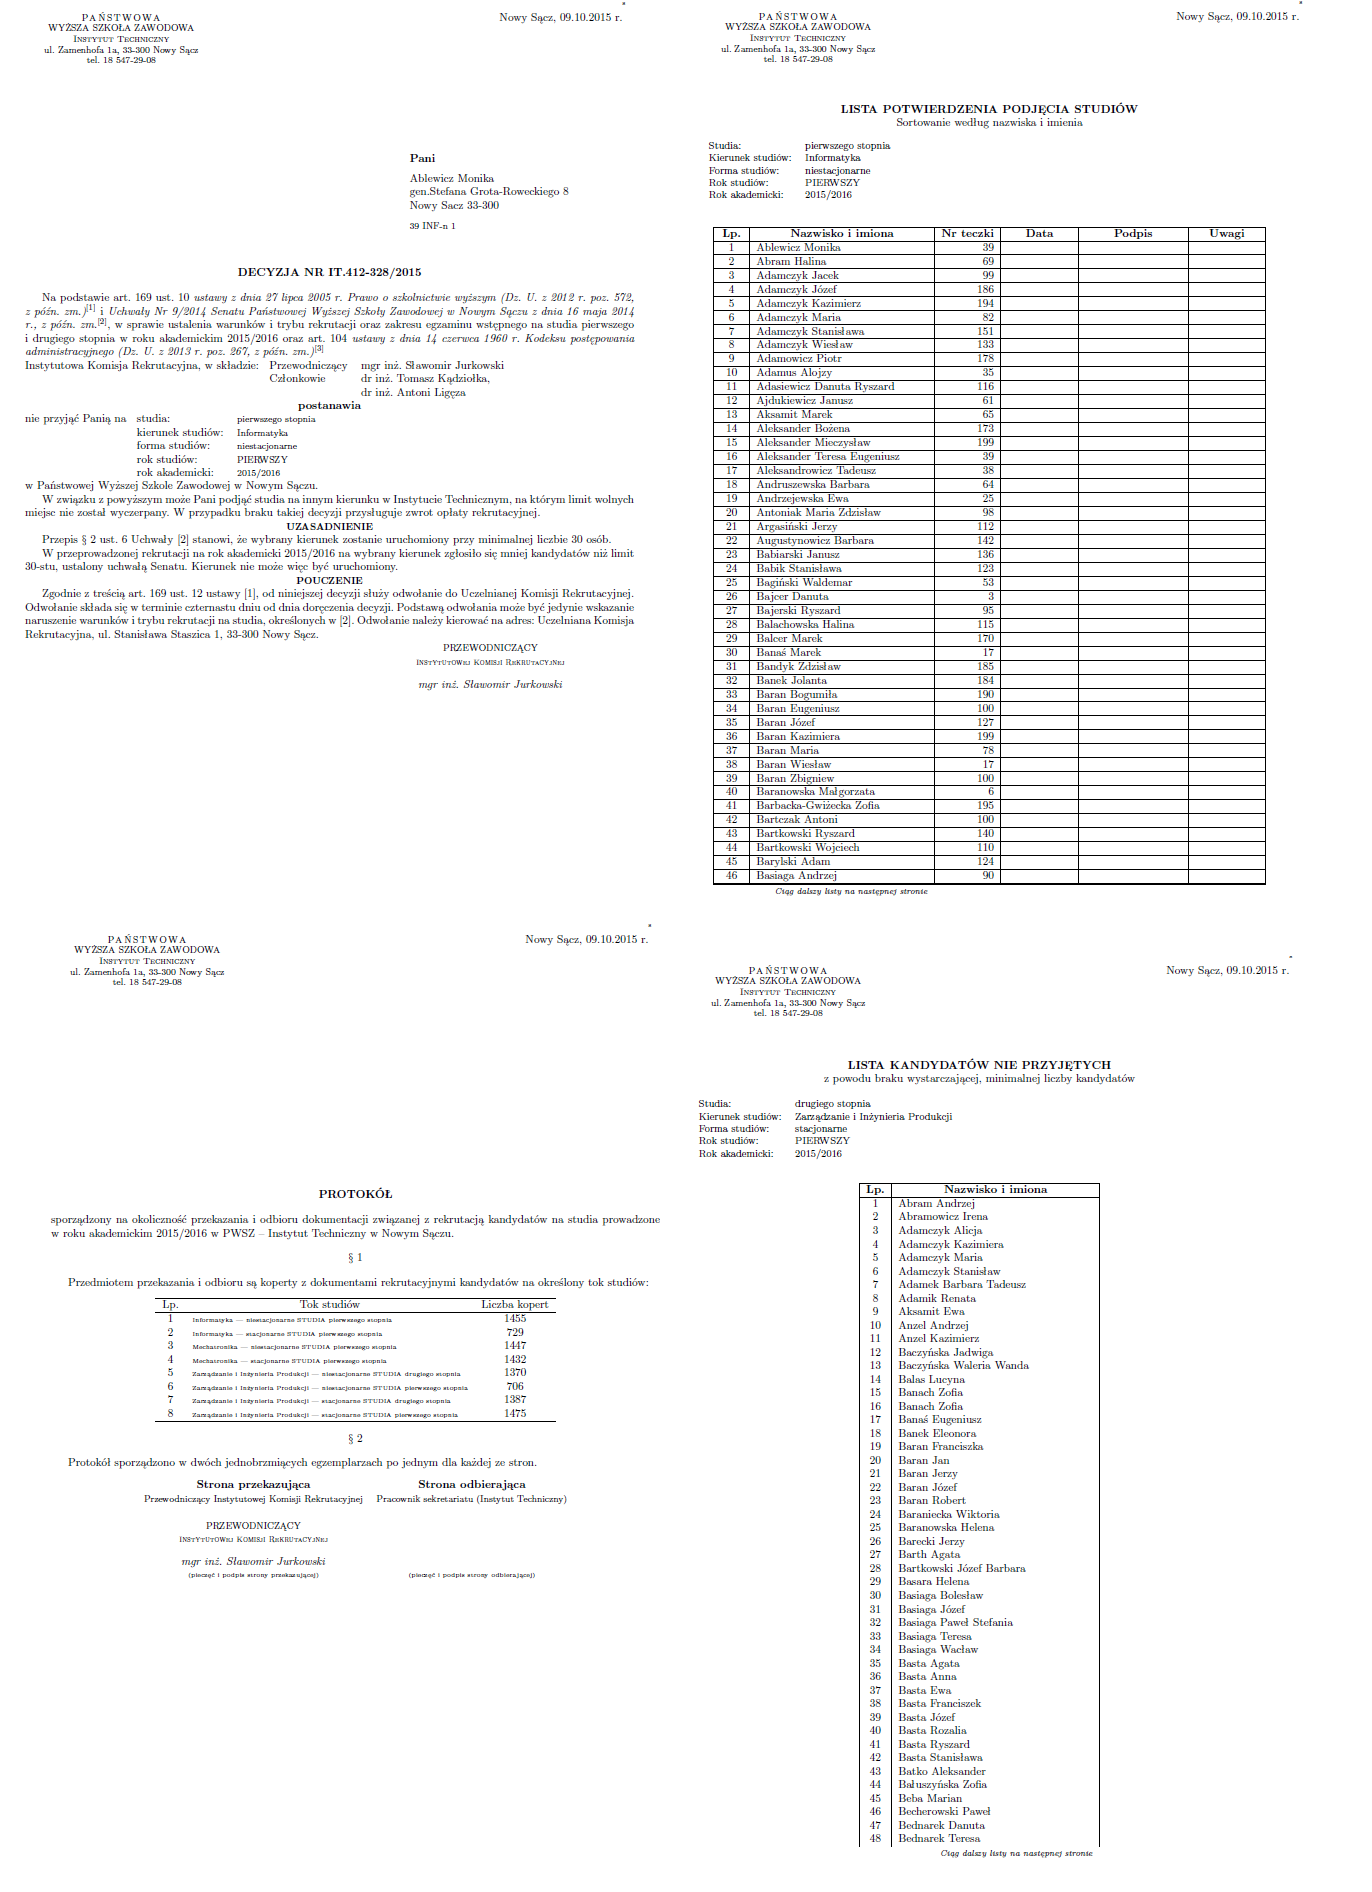
\includegraphics[width=0.8\textwidth]{rys/testy/wynik.png}
    \caption{Przykładowe strony wygenerowanych dokumentów z  testu }
    \label{fig:test}
\end{figure}
\section{Wnioski}
Po udanym przeprowadzeniu testu można stwierdzić, że tak przygotowana paczka systemu raportów zawierająca wszystkie rzeczy do przeprowadzenia rekrutacji, spełnia w pełnym zakresie wymagania postawione w założeniach pracy. Cały katalog roboczy systemu po spakowaniu zajmuje około 50 megabajtów i po rozpakowaniu około 100 megabajtów co oznacza, że przy dzisiejszych nośnikach danych nie będzie problemu z przeniesieniem systemu. Dodatkowo paczka zaraz po rozpakowaniu na systemie Windows jest gotowa do pracy i wymaga jedynie zainstalowanego środowiska uruchomieniowego JAVA 1.8. Cały system tworzenia raportów znajduje się w załączniku 3.


\chapter{Instrukcja obsługi}
DBRaportLatex jest programem napisanym w JAVA'ie służącym do tworzenia raportów w środowisku latex z informacji przechowywanych w bazie danych.
Program ten został przygotowany specjalnie w celu obsługi tworzenia dokumentów potrzebnych do rekrutacji na uczelni PWSZ Nowy Sącz.
Program oparty jest głównie o wcześniej przygotowane szablony w środowisku latex, które w czasie tworzenia raportów są uzupełniane informacjami pobranymi przez program z bazy danych.
Środowisko kompilacji szablonów zostało także przygotowane razem z programem. Kompilacja szablonów jest uruchamiana zaraz po uzupełnieniu szablonów i wynikiem jej jest plik pdf gotowy do wydruku.
\section{Wymagania systemowe}
Program do uruchomienia wymaga zainstalowanego pakietu JAVA 1.8.
\section{Przygotowanie pliku konfiguracyjnego}
zmienne Wprowadza się  za pomocą nazwy zmiennej oraz jej wartości po znaku "=".
Poniżej są opisane wszystkie zmienne:

templatepath - ścieżka do szablonów.
templateoutput - ścieżka do uzupełnionych szablonów(tam zostaną zapisane)
encodingtex - kodowanie zapisu pliku *.tex

dbengine - nazwa sterowników do obsługi danego silnika bazy danych (obsługiwane firebirdsql, mysql)
hostname - IP lub nazwa hosta serwera bazy danych ( //192.168.1.2 lub //Komputer-PC )
port - port serwera bazy danych
dbpath - ścieżka do bazy danych w przypadku firebirda lub nazwa bazy danych w przypadku mysql
user - nazwa użytkownika
password - haslo
dbencoding - kodowanie znaków w bazie danych (może być puste)

pdflatexpath - ścieżka do kompilatora latex
pdflatexpathoutputfolder - ścieżka do skompilowanych plików (PDF)
pdfcompilemainfile - zmienna określająca jakie pliki kompilować za pomocą kompilatora latex. Można tutaj użyć wartości ALL (wszystkie), ONLYBEGDOC (skompilowane zostaną dokumenty tylko z begindoc), NONE (żadne) lub wymienić nazwy plików po przecinku (main.tex,setup.tex ...)
\section{Przygotowanie prostego szablonu}

\section{Polecenia w szablonach}
Uzupelnianie raportow polega na pobraniu przez program z bazy danych rekordow za pomoca przygotowanych wczesniej zapytan SQL zawartych w szablonyach.
Zapytania te nalezy umieszczac na poczatku szablonu w pliku *.tex. Kazde zapytanie to jedna linijka zaczynajaca sie od znaku procetów "%". 
Kazda kolejna linijka ze znakiem "%" bedzie traktowana jako zapytanie do bazy danych az do momentu nowej lini z innym znakiem.
Po tym znaku Piszemy nasze zapytanie z ktorego kazdy rekord bedzie wpisany do szablonu wg metody uzupelnienia ktora jest opisana ponizej.
Kazdy rekord wpisany pod koniec pliku lub miedzy znaczynikami startu i konca dokumentu jezeli one wystepuja w pliku bedzie wpisany wg szablonu:

'\' + nazwa pliku + duza litera numer 1(numer zapytania) + '{' + 1 pole rekordu 1 '}' + '{' + 2 pole rekordu 1  '}' + .. + '{' + n pole rekordu 1 '}'
'\' + nazwa pliku + duza litera numer 1(numer zapytania) + '{' + 1 pole rekordu 2 '}' + '{' + 2 pole rekordu 2  '}' + .. + '{' + n pole rekordu 2 '}'
...
'\' + nazwa pliku + duza litera numer 1(numer zapytania) + '{' + 1 pole rekordu m '}' + '{' + 2 pole rekordu m  '}' + .. + '{' + n pole rekordu m '}'

Dla kolejnych zapytan w jednym szablonie bedzie nadawana kolejna duza litera z alfabetu. Nalezy zauwazyc ze ilosc pól w zapytaniach moze sie roznic.

Przykladowo dla pliku o nazwie szablon(w tabeli vkandydat jest 6 pol i 2 rekordy, w setup 3 pola i 1 rekord):
%SELECT * FROM  vkandydat
%SELECT * FROM  setup

%\szablonA{Pawel}{Mysinski}{Przyjety}{1000}{STACJONARNE}{INFORMATYKA}
%\szablonA{Mateusz}{Mroz}{Przyjety}{1000}{STACJONARNE}{INFORMATYKA}

%\szablonB{2014}{jakis_text}{blablabla}


Ograniczenie zapytan w jednym szablonie jest jak widac do 26 tyle ile liter w alfabecie.
Ograniczenie pol dla zapytania jest narzucone przez Latex i jest to 9 pol natomiast program wyrzuci wiecej i moze to spowodowac problem przy kompilacji szablonu.
\subsection{Polecenie puste}

\subsection{Grupowanie}
Istnieje takze mozliwosc w programie grupowania po polach od ktorych zaczyna sie zapytanie. Zapis grupowania jest niezalezne od zapisu grupwania, natomiast dzialanie wymaga pewnego dodatku do zapytania jakim jest ordering.
Zapis grupowania:
%`a,b,c,d,...`SELECT ........ ORDER BY ....
'`' - nie mylic z apostrofem (tylda bez shift'a)
a,b,c,d,... - to liczby naturalne, ktore oznaczaja na ilu polach bedzie oparta grupa. grup moze byc od 1 do 26 i oparta maksymalnie na 9 polach.
ORDER BY .... - Zaznaczyc trzeba ze przed grupowaniem nalezy uporzatkowac rekordy wedlug pol po ktorych grupujemy inaczej grupy moga sie powtorzyc co zpowoduje zly wydruk danych.
Grupowanie dziala wedlug zasad:
Z pobranych rekordow z bazy danych zabierane sa te pola ktore sa grupowane i wrzucane do danej grupy o unikalnych swoich wartosciach. 
Ostateczne rekordy beda mialy tylko te wartosci pol ktore nie byly grupowane.
Kazda grupa bedzie otwarta i zamknieta.
Grupy nie przeplataja sie.
Zapytania z grupowaniem sa niezalezne tak samo jak kazde inne zapytanie i mozna je mieszac z innymi zapytaniami.

Struktura odnosnie nazewnictwa odnosnie ktore z kolei jest to zapytanie jest zachowana. Dodana jest natomiast struktura grup:
%nazwy dla poczatku grupy: '\' + nazwapliku + duza litera (wg numer zapytania)+ duza litera wg nr grupy +  "{" + wartosc 1 po zgrupwaniu + "}" + ... +"{" + wartosc n po zgrupwaniu + "}"
%Snazwy dla konca grupy: '\' + "end" + nazwapliku + duza litera (wg numer zapytania) + duza litera wg nr grupy +  "{" + wartosc 1 po_zgrupwaniu + "}" + ... +"{" + wartosc n po zgrupwaniu + "}" 
\section{Uruchomienie programu}
\section{Rozwiązywanie problemów}

\chapter{Podsumowanie}
Opracowany system generowania raportów usprawni i przyspieszy wszelkie procesy, w których możliwa jest automatyzacja tworzenia dokumentów. Rozpoczęcie tworzenia systemu było głównie z myślą o obsłudze rekrutacji na uczelni PWSZ Nowy Sącz na wydziale Technicznym, jednak w czasie realizacji projektu koncepcja ta została zastąpiona pełnym uogólnieniem możliwości do których może on służyć. Dzięki temu stworzony system można wykorzystać, w każdym przypadku generowania dokumentów, w którym możliwe jest utworzenie szablonu w środowisku LaTeX.
\vspace{5mm}
\par
Projekt wcześniej przeszedł pozytywnie testy na wygenerowanych danych, które w wyczerpujący sposób sprawdziły funkcjonalność programu, co dało pełną gwarancję niezawodności przy zastosowaniu go przy tworzeniu dokumentów podczas rekrutacji na uczelni.
\vspace{5mm} 
\par
Dzięki szablonom dokumentów, potrzebnych przy procesie rekrutacji, przygotowanych razem z programem, system z łatwością został wykorzystany przy rekrutacji na uczelni PWSZ Nowy Sącz, na wydziale Technicznym, w 2015 roku, na semestr zimowy i sprawdził się bezbłędnie. 
\vspace{5mm}
\par
Dzięki programowi DBLatexRaport stworzonemu na potrzeby pracy jest możliwe:\vspace{5mm}
\begin{itemize}
\item pełna automatyzacja procesu tworzenia dokumentów oraz raportów przy pomocy wcześniej stworzonych szablonów.\vspace{5mm}
\item usprawnienie pracy przy segregowaniu raportów\vspace{5mm}
\item znaczny wzrost prędkości przebiegu całego procesu.\vspace{5mm}
\item eliminacja błędów człowieka, które mogły powstać przy ręcznym tworzeniu raportów.\vspace{5mm}
\item ze względu na kompatybilność z wieloma silnikami bazodanowymi, uruchomienie programu z różnych źródeł danych (jeśli źródło danych posiada bibliotekę JDBC).\vspace{5mm}
\item ze względu na fakt iż program jest napisany w języku JAVA 1.8, uruchomienie go na wielu systemach operacyjnych, które mają możliwość zainstalowania pakietu JAVA.\vspace{5mm}
\end{itemize}\vspace{5mm}
\par
Do programu dołączona jest krótka instrukcja obsługi, dzięki której każdy będzie w stanie skonfigurować i uruchomić program. Jedynym wymaganiem sprawnego użytkowania programu jest umiejętność pisania dokumentów w systemie LaTeX, aby móc stworzyć szablony raportów.
\vspace{5mm}
\par 
Biorąc pod uwagę powyższe stwierdzenia, można uznać, że osiągnięto cel postawiony  w pracy.
\appendix

% tutaj załączniki

%\chapter*{Bibliografia}
\nocite{*}
\bibliographystyle{plplain}
%\bibliographystylebk{plplain}
%\bibliographystylest{plplain}
%\bibliographystyledoc{plplain}
% \bibliographystyleweb{plplain}
%\bibliographybk{BIB/books}
%\bibliographyst{BIB/books}
%\bibliographydoc{BIB/books}
% \bibliographyweb{BIB/books}

% \bibliography{bib/verificard,bib/jml,bib/daikon}
\bibliography{bib/daikon,bib/statistics,bib/other}

\end{document}

% ex: set tabstop=4 shiftwidth=4 softtabstop=4 noexpandtab fileformat=unix filetype=tex spelllang=pl,en spell:

